\documentclass[a4paper]{report}
\usepackage[utf8]{inputenc}
\usepackage[T1]{fontenc}
\usepackage{RJournal}
\usepackage{amsmath,amssymb,array}
\usepackage{booktabs}


% tightlist command for lists without linebreak
\providecommand{\tightlist}{%
  \setlength{\itemsep}{0pt}\setlength{\parskip}{0pt}}

\usepackage{longtable}

% Always define CSL refs as bib entries are contained in separate doc
% Pandoc citation processing
\newlength{\cslhangindent}
\setlength{\cslhangindent}{1.5em}
\newlength{\csllabelwidth}
\setlength{\csllabelwidth}{3em}
\newlength{\cslentryspacingunit} % times entry-spacing
\setlength{\cslentryspacingunit}{\parskip}
% for Pandoc 2.8 to 2.10.1
\newenvironment{cslreferences}%
  {}%
  {\par}
% For Pandoc 2.11+
\newenvironment{CSLReferences}[2] % #1 hanging-ident, #2 entry spacing
 {% don't indent paragraphs
  \setlength{\parindent}{0pt}
  % turn on hanging indent if param 1 is 1
  \ifodd #1
  \let\oldpar\par
  \def\par{\hangindent=\cslhangindent\oldpar}
  \fi
  % set entry spacing
  \setlength{\parskip}{#2\cslentryspacingunit}
 }%
 {}
\usepackage{calc}
\newcommand{\CSLBlock}[1]{#1\hfill\break}
\newcommand{\CSLLeftMargin}[1]{\parbox[t]{\csllabelwidth}{#1}}
\newcommand{\CSLRightInline}[1]{\parbox[t]{\linewidth - \csllabelwidth}{#1}\break}
\newcommand{\CSLIndent}[1]{\hspace{\cslhangindent}#1}


\usepackage[labelformat=simple]{subcaption}
\renewcommand\thesubfigure{(\alph{subfigure})}
\usepackage{tikz,enumitem}
\usetikzlibrary{positioning, arrows.meta, shapes.geometric}
\tikzset{%
  semithick,
  >={Stealth[width=2mm, length=2.75mm]},
  obs/.style = {name = #1, circle, draw, inner sep = 5pt, label = center:\(\scriptstyle#1\)},
  fixed/.style = {name = #1, regular polygon, regular polygon sides = 4, draw, inner sep = 3pt, label = center:\(#1\)},
  lat/.style 2 args = {name = #1, circle, draw, dashed, inner sep = 5pt, label = center:\(\scriptstyle#2\)},
}
%\newtheorem{lemma}{Lemma}
\newcommand\independent{\protect\mathpalette{\protect\independenT}{\perp}}
\def\independenT#1#2{\mathrel{\rlap{\(#1#2\)}\mkern2mu{#1#2}}}
\newcommand{\+}[1]{\ensuremath{\mathbf{#1}}}
\newcommand{\doo}{\textrm{do}}


\begin{document}


%% do not edit, for illustration only
\sectionhead{Contributed research article}
\volume{15}
\volnumber{3}
\year{2023}
\month{September}
\setcounter{page}{26}

\begin{article}
  % !TeX root = RJwrapper.tex
\title{SSNbayes: An R Package for Bayesian Spatio-Temporal Modelling on Stream Networks}


\author{by Edgar Santos-Fernandez, Jay M. Ver Hoef, James McGree, Daniel J. Isaak, Kerrie Mengersen, and Erin E. Peterson}

\maketitle

\abstract{%
Spatio-temporal models are widely used in many research areas from ecology to epidemiology. However, a limited number of computational tools are available for modeling river network datasets in space and time. In this paper, we introduce the \texttt{R} package \href{https://CRAN.R-project.org/package=SSNbayes}{SSNbayes} for fitting Bayesian spatio-temporal models and making predictions on branching stream networks. \href{https://CRAN.R-project.org/package=SSNbayes}{SSNbayes} provides a linear regression framework with multiple options for incorporating spatial and temporal autocorrelation. Spatial dependence is captured using stream distance and flow connectivity while temporal autocorrelation is modelled using vector autoregression approaches. \href{https://CRAN.R-project.org/package=SSNbayes}{SSNbayes} provides the functionality to make predictions across the whole network, compute exceedance probabilities, and other probabilistic estimates, such as the proportion of suitable habitat. We illustrate the functionality of the package using a stream temperature dataset collected in the Clearwater River Basin, USA.
}

\section{Introduction}

Rivers and streams are of vital ecological and economic importance \citep{vorosmarty2010global} but are under pressure from anthropogenic impacts such as climate change, pollution, water extractions, and overfishing. In the past, data describing critical characteristics such as nutrients, sediments, pollutants and stream flow tended to be sparse in space and/or time. However, recent developments in in-situ sensor technology have revolutionized ecological research and natural resource monitoring. These new data sets create exciting opportunities to measure, learn about, and manage the spatio-temporal dynamics of abiotic (e.g. temperature, water chemistry, habitat characteristics) and biotic processes (e.g. migration, predation, and competition). However, the unique spatial relationships found in stream data (e.g. branching network structure, longitudinal (upstream/downstream) connectivity, water flow volume and direction) and high-frequency of sampling create analytical challenges that make it difficult to gain meaningful insights from these datasets. We attempt to overcome these challenges through the \CRANpkg{SSNbayes} package which provides convenient and practical tools to undertake Bayesian inference in complex spatial and temporal stream network settings.  



\subsection{Motivating dataset: repeated measures from \emph{in-situ} sensor locations in a river}
\label{sec:motiv}

Consider the river network in the Clearwater River Basin, USA shown in Fig~\ref{figure:net}. 
Water temperature data were collected at fixed time intervals using in-situ sensors placed at 18 unique locations throughout the network \citep{isaak2018principal}. 
We want to use these data to address several research questions and goals.
Firstly, we would like to analyse water temperature to assess the impact of covariates such as air temperature. 
Secondly, we aim to make predictions with uncertainty at other locations throughout the network (approximately every 1 km). 
Also, we want to impute missing data e.g. the most downstream point in Fig~\ref{figure:net} (location 12), and determine regions of the network which remain suitable habitats over time to sustain fish species such as bull trout which typically preferred water temperatures of < 13 \textdegree{}C.  
Throughout this paper, we show how the \CRANpkg{SSNbayes} package can be used to analyse these spatial and temporal data, and address these motivating research questions.

 

\begin{figure}[htb]
  \centering
   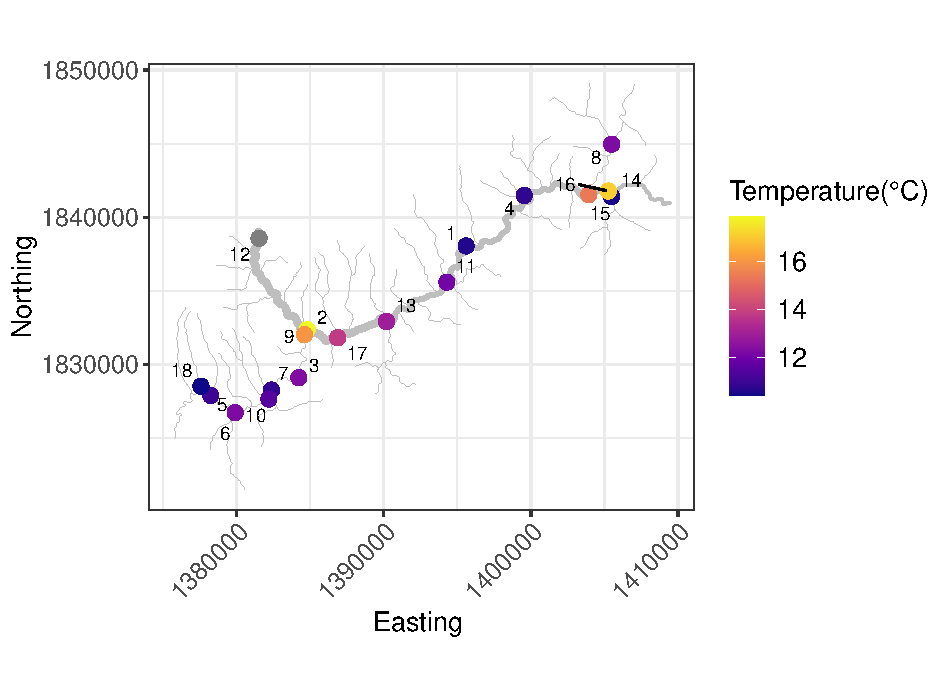
\includegraphics[width=4.5in]{./Figs_Pay/net.pdf}
  \caption{%Clearwater's stream network 
 Mean daily water temperature in degrees Celsius on August 1, 2012, at 18 different spatial locations in the Clearwater stream network in the US. The temperature values are represented by a color scale, with cooler temperatures shown in blue and warmer temperatures shown in yellow. Each spatial location is labeled with a unique identifier (\texttt{locID}). The plot highlights the variation in water temperature across the different locations in the network.
 % Mean daily water temperature in C$^{\circ}$ for 2012-08-01 at 18 spatial locations in the Clearwater stream network.  The labels specify the location identifier (\texttt{locID}).
 } 
  \label{figure:net}
\end{figure}


\subsection{A brief review}
\label{sec:review}

A number of \textsf{R} software packages for spatial stream-network modelling have been developed over the last few decades \citep{hoef2014ssn, rtop, smnet}.
These packages account for unique spatial relationship found in stream data.
For example, the \textsf{R} packages \CRANpkg{SSN} and \CRANpkg{SSN2} \citep{hoef2014ssn, SSN2} fits spatial regression models for stream networks, with autocorrelation in time only possible by using random effects as repeated measures, which induces equal correlation for all times at a location. Similarly, spatial additive models can be fitted using the package \CRANpkg{smnet} \citep{smnet}.
However, these models are not designed to simultaneously account for the temporal variability that often accompanies spatial variation in new data sets derived from modern sensor arrays. 


There are several \textsf{R} packages for spatio-temporal modelling that are described in the Space-time CRAN Task View \citep{cranSpaceTime}. For example, spatial/temporal dependence can be incorporated via the \CRANpkg{nlme} package  package \citep{nlmeBook, nlme}. 
Other packages such as \CRANpkg{spBayes} \citep{spBayes} allow random effects modelling for point-referenced data. 
\CRANpkg{CARBayes} \citep{CARBayes} contains useful tools for implementing Bayesian spatial models using random effects via conditional autoregressive (CAR) priors. 
Similarly, spatial process data can be represented using kernels
e.g. using the package \pkg{RandomFields}  \citep{RandomFields}. 
Interpolation of spatial data and Kriging can be done via tools from the package \CRANpkg{geoR} \citep{geoR}. 
One of the most popular implementations among practitioners is the \pkg{R-INLA} package \citep{rinla}, which uses approximate Bayesian inference via integrated nested Laplace approximations. 
Multiple latent Gaussian spatio-temporal models can be fit in \pkg{R-INLA}. 
\CRANpkg{FRK} \citep{FRKpaper} makes use of spatial basis functions and discrete areal units with a focus on large datasets. 
In the same line, new packages harnessing the power of \CRANpkg{rstan} \citep{carpenter2017stan} are also emerging. For instance, \CRANpkg{bmstdr} \citep{bmstdr} implements several spatio-temporal approaches for point referenced and areal unit datasets, and \CRANpkg{geostan}  \citep{geostan} fits spatial models for areal data.    
However, none of these packages are specifically designed to account for the unique spatial relationships found in data collected on streams.  

Here, we describe the \CRANpkg{SSNbayes} package which has been designed to address many of the limitations of the current software tools for spatio-temporal modelling on stream networks. More specifically, \CRANpkg{SSNbayes} can fit spatio-temporal stream-network models and produce predictions in space and time, with associated estimates of uncertainty. It uses the Bayesian inference machinery implemented using the probabilistic programming language \textsf{Stan}. 

The rest of the paper is organised as follows: we introduce the relevant statistical models in the Methods section, followed by an overview of the package structure and functions. We then demonstrate how the \CRANpkg{SSNbayes} package can be used to explore, analyse and draw conclusions from a stream temperature data set collected in the western United States (USA). A second reproducible example is provided in the Appendix to help users adapt the \textsf{R} code for their own data. Finally, we conclude with a discussion of the benefits and challenges in using the \CRANpkg{SSNbayes} package and Bayesian spatio-temporal models on stream networks, as well as potential extensions to the methods and improvements to the package.



\section{Methods}
\label{sec:met}

Data collected on stream networks often exhibit complex patterns of spatial autocorrelation resulting from ecosystem processes occurring within branching stream networks, as well as between the aquatic and terrestrial environments \citep{peterson2013modelling}. 
It is therefore common for streams data to exhibit \textit{both} Euclidean and in-stream patterns of spatial autocorrelation at multiple scales \citep{peterson2006patterns, peterson2010mixed}. Thus, we start this section with a description of spatial models based on Euclidean distance and then describe methodological extensions to stream networks. These models provide the foundation to describe the Bayesian hierarchical spatio-temporal model variations implemented in the \CRANpkg{SSNbayes} package. 

\noindent 
\subsection*{General space-time model}

Consider the general spatio-temporal linear model:

\begin{equation}
\pmb{y} = \pmb{X}\pmb{\beta} + \pmb{v} + \pmb{\epsilon},
\label{eq:lm0}
\end{equation}

\noindent where the response variable $\pmb{y} = [\pmb{y}_1^{'}, \pmb{y}_2^{'},\cdots,\pmb{y}_T^{'}]^{'}$ is a stacked vector of length $n = S\times T$ for $S$ spatial locations and $T$ time points. 
We order data such that vector $\pmb{y}_t$ contains the observations at the $S$ spatial locations at time $t$ for $t = 1, \ldots, T$.
Let $\pmb{X_t}$ be an $S \times p$ design matrix of $p$ covariates for the $t$th time.
We construct a stacked matrix of covariates 
$\pmb{X} = [\pmb{X}_1^{'}, \pmb{X}_2^{'},\cdots,\pmb{X}_T^{'}]^{'}$ with dimensions $n \times p$. 
We then define $\pmb{\beta}$ as a $p \times 1$ vector of regression coefficients.
We let $\pmb{v} = [\pmb{v}_1^{'}, \pmb{v}_2^{'},\cdots,\pmb{v}_T^{'}]^{'}$ be a stacked vector of $n$ spatial random effects, where $\pmb{v}_t$ is a  vector of length $S$ for each $t$, and all $\pmb{v}_t$ have the same spatial dependence model (shared locations and parameters across all times $t$). For example, $\pmb{v}_t$ can be modelled using a Gaussian process \citep{banerjee2014hierarchical}, but we also use spatial stream-network models that we describe below for each $\pmb{v}_t$. The final step in our construction is to use vector autoregressive models to add the temporal components which we develop below. %among $\{\pmb{v}_t\}$,
The vector $\pmb{\epsilon}$ is the independent unstructured random error term, where $\textrm{var}(\pmb{\epsilon}) = \sigma^2_0\pmb{I}$. The parameter $\sigma_{0}^2$ is called the nugget effect and $\pmb{I}$ is an $n \times n$ identity matrix.


\subsection*{Euclidean distance models}

A typical modelling approach to capture spatial dependence is via the second moment of $\pmb{v}$ from Eq~\ref{eq:lm0} where the amount of autocorrelation decays with the Euclidean distance. 
Some of the most common covariance functions are the exponential, Gaussian and spherical \citep{cressie2015statistics, banerjee2014hierarchical}: 


\begin{equation}
    \textrm{exponential model,} \ \  C_{ED}(d\mid \pmb{\theta}) = \sigma_e^2 e^{-3d/\alpha_e},
    \label{eq:ced}
\end{equation}
\begin{equation}
    \textrm{Gaussian model,} \ \ C_{ED}(d\mid \pmb{\theta}) = \sigma_e^2 e^{-3(d/\alpha_e)^2},
\label{eq:ced2}
\end{equation}
and
\begin{equation}
\textrm{spherical model,} \ \ C_{ED}(d\mid \pmb{\theta}) = \sigma_e^2\left(1-\frac{3d}{2\alpha_e} + \frac{d^3}{2\alpha_e^3}\right)\mathbbm{1}(d/\alpha_e \leqslant 1),
\label{eq:ced3}
\end{equation}


\noindent where $\alpha_e \in (0,\infty), \sigma_e ^ 2 > 0$, and $d$ is the Euclidean distance between two locations $s_i$ and $s_j$.
The vector $\pmb{\theta}$ represents the spatial parameters ($\alpha_e$, $\sigma_e^2$), where 
$\sigma_e^2$ is the partial sill, $\alpha_e$ is the spatial range parameter and $\mathbbm{1}(\cdot)$ is the indicator function. 
The partial sill is the resulting variance after accounting for the nugget effect (sill minus nugget effect).
Negligible spatial correlation is assumed between points located at a distance greater than the spatial range parameter.  



\subsection{Spatial models for stream networks}

The stream network data shown in Fig.\ref{fig:network} represents repeated measures at several time points $t$ from four spatial locations ($s_1$ to $s_4$). Stream distance is defined as the separation distance between two locations when movement is restricted to the network. The direction of the water flow is also shown in the figure (from north to south) and the stream outlet (i.e. most downstream point on the stream network) is below location $s_4$. The watershed (i.e. drainage basin) includes the land that contributes water flow to a discrete downstream location in the stream network. Thus, the watershed for the stream outlet in Fig. \ref{fig:network} includes all of the upstream regions ($r_1$-$r_4$). Spatial locations $s_1$ and $s_3$ are considered flow-connected because the water flows from the upstream location $s_1$ to the downstream location $s_3$. In contrast, $s_1$ and $s_2$ are considered flow-unconnected because they reside on the same stream network, but do not share flow. 
% The distances from each site in a pair of flow-unconnected locations to the junction are defined as $a$ and $b$, where $a \leqslant b$.

\begin{figure}[htbp]
  \centering
   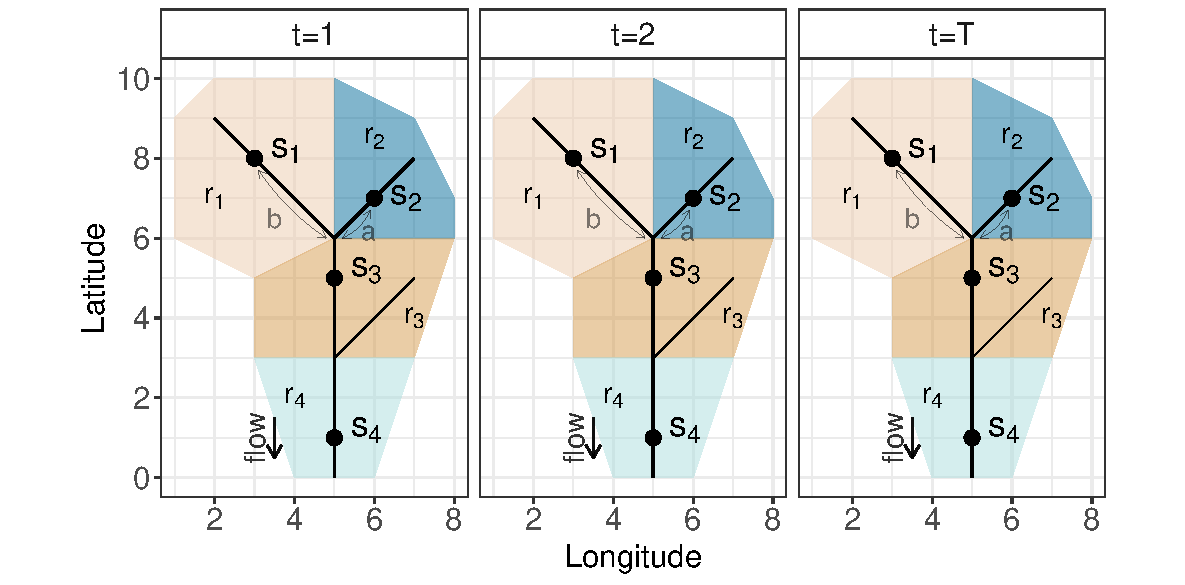
\includegraphics[width=5.25in]{./Figs_Pay/netw.pdf}
  \caption{
  %Stream network across multiple time points. Four spatial locations ($s_1-s_4$) and four regions ($r_1-r_4)$ are depicted. 
 Visualization of a stream network at multiple time points, with water flowing from top to bottom. The plot displays four spatial locations ($s_1-s_4$) and four regions ($r_1-r_4)$, with the colors indicating the regions. This visualization allows for an understanding of the spatial and temporal dynamics of the stream network.  
  }
  % Fig produced by file 000 network points fig paper.R 
  \label{fig:network}
\end{figure}

Multiple covariance models have been proposed for stream networks that describe the unique spatial dependence related to network structure and stream flow. These models are based on moving average constructions that use stream distance, and were introduced by \citet{ver2006spatial} and \citet{cressie2006spatial} (tail-up models) and \citet{ver2010moving} and \citet{garreta2010spatial} (tail-down models); several models of each class are given below. These spatial covariance matrices have been extensively employed in numerous water quality modelling frameworks and applications \citep{money2009using, money2009modern, isaak2014applications, mcmanus2020variation, jackson2018spatio, rodriguez2019spatial} and are described in more detail below. 



\subsubsection{Tail-up models}
Tail-up covariance models were developed by convolving a moving average function with white noise \citep{ver2006spatial}. As the name suggests, the moving average function points in the upstream direction from a stream location in a tail-up model, which restricts correlation to flow-connected locations only. In addition, the function must be split at upstream junctions using spatial weights, which maintain stationary variances by controlling the proportion allocated to each upstream segment.

Given a pair of sites $s_i$ and $s_j$, the tail-up covariance matrix is defined as:

$$C_{TU}(s_i,s_j|\pmb{\theta}) = \left\{\begin{matrix}
0 \:\:\: \textrm{if $s_i,s_j$ are flow-unconnected}, \\C_u(h\mid \pmb{\theta}) W_{ij} \:\:\: \textrm{if $s_i,s_j$ are flow-connected}, \end{matrix}\right.$$

\noindent where $C_u(h\mid \pmb{\theta})$ is an unweighted tail-up covariance between two locations based on the total stream distance between them, $h$. $W_{ij}$ represents the spatial weights between sites $i$ and $j$. $C_u$ can take a variety of forms including:


\begin{align}
\textrm{Tail-up exponential model},& \ \ C_{u}(h \mid \pmb{\theta}) = \sigma_u^2 e^{-3h/\alpha_u}, \\
\textrm{Tail-up linear-with-sill model},& \ \ C_u(h \mid \pmb{\theta}) = \sigma_u^2 (1-h/\alpha_u)\mathbbm{1}(h/\alpha_u \leqslant 1), \\
\textrm{Tail-up spherical model},& \ \ C_u(h \mid \pmb{\theta}) = \sigma_u^2 \left(1-\frac{3h}{2\alpha_u} + \frac{h^3}{2\alpha_u^3}\right)\mathbbm{1}(h/\alpha_u \leqslant 1)
\end{align}

\noindent where $\sigma^2_{u}$ is the partial sill and $\alpha_u$ is the range parameter.

The spatial weights used in the tail-up model are generated for flow-connected locations 

$$W_{ij}=\sqrt[]{\frac{\Omega(s_j)}{\Omega(s_i)}},$$

\noindent where $\Omega(s_i)$ and $\Omega(s_j)$ are the additive function values for the upstream and downstream site, respectively. Additive function values can be derived from any variable available for every line segment in a stream network, but are often based on an ecologically meaningful variable (e.g. stream flow) or a surrogate (e.g. watershed area), which is thought to represent relative influence in a stream network \citep{frieden2014improving}. Additive function values can be generated in \CRANpkg{SSN} using the \texttt{additive.function()} or in the STARS ArcGIS custom toolset using the \texttt{SegmentPI}, \texttt{Additive Function - Edges}, and \texttt{Additive Function - Sites} tools \citep{peterson2014stars}. For additional information about how the additive function values are constructed, please see \citet{ver2006spatial} or Appendices A in \citet{santos2022bayesian} or \citet{peterson2010mixed}. 

\subsubsection{Tail-down models}
Tail-down models are also based on a moving average contruction \citep{ver2010moving}, but in this case the function points in the downstream direction. This allows the models to describe spatial correlation between both flow-connected and flow-unconnected locations. In addition, the moving average functions converge downstream and do not need to be split at junctions using spatial weights. 

There is a distinction between flow-connected and flow-unconnected relationships in a tail-down model. When pairs of sites are flow-connected, distance is based on the total stream distance between them, $h$. When sites are flow-unconnected (e.g. $s_1$ and $s_2$ in Fig.\ref{fig:network}), we define $a$ and $b$ as the stream distance from $s_1$ and $s_2$ to their first common downstream junction,  so that $a \leqslant b$. 

Tail-down exponential model,
%
$$C_{TD}(a,b, h|\pmb{\theta}) = \left\{\begin{matrix}
\sigma_d^2 e^{-3h/\alpha_d} \:\:\: \textrm{if flow-connected,} \\
\sigma_d^2 e^{-3(a+b)/\alpha_d} \:\:\: \textrm{if flow-unconnected,} \end{matrix}\right. $$
%
Tail-down linear-with-sill model,
%
$$C_{TD}(a,b, h|\pmb{\theta}) = \left\{\begin{matrix}
\sigma_d^2 (1-\frac{h}{\alpha_d})\mathbbm{1}(\frac{h}{\alpha_d} \leqslant 1) \:\:\: \textrm{if flow-connected,} \\
\sigma_d^2 (1-\frac{b}{\alpha_d})\mathbbm{1}(\frac{b}{\alpha_d} \leqslant 1) \:\:\: \textrm{if flow-unconnected,} \end{matrix}\right. $$
%
Tail-down spherical model,
%
$$C_{TD}(a,b, h|\pmb{\theta}) = \left\{\begin{matrix}
\sigma_d^2 (1-\frac{3h}{2\alpha_d} + \frac{h^3}{2\alpha_d^3})\mathbbm{1}(\frac{h}{\alpha_d} \leqslant 1) \:\:\: \textrm{if flow-connected,}\\
\sigma_d^2 (1-\frac{3a}{2\alpha_d} + \frac{b}{2\alpha_d})(1-\frac{b}{\alpha_d})\mathbbm{1}(\frac{b}{\alpha_d} \leqslant 1) \:\:\: \textrm{if flow-unconnected,} \end{matrix}\right. $$
%
where $\sigma_d^2$ is the partial sill, $\alpha_d$ is the range parameter, and $\mathbbm{1}(\cdot)$ is the indicator function, equal to 1 if its argument is true, otherwise it is zero.

\subsection{Mixed models}
A mixture of Euclidean, tail-up and tail-down covariance matrices is often used to capture the complex patterns of spatial dependency found in stream data. In Eq~\ref{eq:lm0}, $\pmb{v}_t$ for a purely spatial case is a vector of dimension $S$ corresponding to the spatial locations, with covariance matrix $\pmb{\Sigma}$.


\begin{equation}
\pmb{\Sigma} = COV(\pmb{v}) = \pmb{C}_{ED} + \pmb{C}_{TU} + \pmb{C}_{TD}   
= \sigma_e^2\pmb{R}_{e}(\alpha_e)+\sigma_u^2\pmb{R}_{u}(\alpha_u) + \sigma_d^2\pmb{R}_{d}(\alpha_d), %+ \sigma_d^{2}_{0}\pmb{I} 
%+ \sigma_d^2_0\pmb{I}
\label{eq:covs}
\end{equation}



\noindent where $\sigma^2_{e}$, $\sigma^2_{u}$, and $\sigma^2_{d}$ are the partial sills for Euclidean, tail-up and tail-down functions, respectively. The correlation matrices $\pmb{R}_{u}(\alpha_u)$, $\pmb{R}_{d}(\alpha_d)$ and $\pmb{R}_{e}(\alpha_e)$ are obtained as a function of the range parameters $\alpha_u$, $\alpha_d$ and $\alpha_e$ \citep{hoef2014ssn}.

For space-time applications, we can use the same spatial covariance matrix or we can build a dynamic model with spatial parameters that are time-specific. We opted for the first approach in the \CRANpkg{SSNbayes}, since this reduces the number of parameters to be estimated from the model and is less computationally demanding. We return to this point in the Discussion.


\subsection{Spatio-temporal stream network models}

Following the above discussion, consider the stream network in Fig.\ref{fig:network}, that evolves across discrete time points $t = 1, 2, \ldots, T$.
Let a response variable $\pmb{y}_t$ be an $S \times 1$ vector of random variables at unique and fixed spatial locations of $s = 1, 2, \ldots, S$. 
We start with the following conditional spatio-temporal model:

\begin{equation}
[\pmb{y}_1,\pmb{y}_2,\cdots,\pmb{y}_T] =  \prod_{t=2}^{T}[\pmb{y}_t \mid  \pmb{y}_{t-1}, \pmb{\theta},\pmb{X}_{t},\pmb{X}_{t-1},\pmb{\beta}, \pmb{\Phi}, \pmb{\Sigma}]%[\pmb{y}_1] 
\label{eq:VAR1def}
\end{equation}
where $\pmb{y}_1$ is the process at $t=1$, and
\begin{equation}
[\pmb{y}_t \mid  \pmb{y}_{t-1},\pmb{\theta},\pmb{X}_{t},\pmb{X}_{t-1},\pmb{\beta}, \pmb{\Phi}, \pmb{\Sigma}  ] \sim \mathcal{N}(\pmb{\mu}_{t},\pmb{\Sigma} + \sigma^2_0\pmb{I}), 
\end{equation}

\noindent Here, $\pmb{\Sigma} = COV(\pmb{v}_t)$ is an $S \times S$ spatial covariance matrix of the form given in Eq~\ref{eq:covs}.
The mean $\pmb{\mu}_{t}$ can be expressed as a vector autoregressive process of order one VAR(1) \citep{hamilton1994time}:

\begin{equation}
\pmb{\mu}_{t} = \pmb{X}_{t}\pmb{\beta} + \pmb{\Phi} (\pmb{y}_{t-1} - \pmb{X}_{t-1}\pmb{\beta}),
\label{eq:err_}
\end{equation}

\noindent The square transition matrix, $\pmb{\Phi}$ of dimension $S \times S$, has elements $\phi_{ij}$, which describe the conditional temporal cross-correlation between two spatial locations $i$ and $j$. 



\subsection {Vector autoregressive model variations}
\label{sec:dst}

We use a vector autoregressive (VAR) approach to simultaneously model time series from multiple spatial locations in the network. This stochastic approach allows capturing and incorporating temporal dependence across multiple time series.  
Two variations of the vector autoregressive spatial process have been implemented in the \CRANpkg{SSNbayes} package.

\noindent {\bf Case 1 (AR)}

\noindent The simplest case considers the same temporal autocorrelation for all spatial locations. Therefore all the diagonal elements of $\pmb{\Phi}$ are equal to $\phi$ and all the off-diagonal elements are set to zero, which assumes negligible cross-correlation between time series. That is:

\begin{equation}\label{eq:case1}
\pmb{\Phi} = \begin{bmatrix}
\phi & 0 & \cdots & 0 \\ 
0 & \phi &  \cdots  & 0 \\ 
\vdots & \vdots &  \ddots & \vdots \\ 
0 & 0  & \cdots & \phi \\
\end{bmatrix}.
\end{equation}
Under this model, the temporal autocorrelation for a fixed spatial location is an AR1 model with autocorrelation parameter $\phi$, and the joint spatio-temporal autocovariance matrix is the separable model,

\begin{equation}\label{eq:separable}
\textrm{var}({\mathbf{y}}) = \pmb{C}_{OO} =
\frac{1}{1 - \phi^2}\begin{bmatrix}
1 & \phi & \cdots & \phi^{T-1} \\ 
\phi & 1 &  \cdots  & \phi^{T-2} \\ 
\vdots & \vdots &  \ddots & \vdots \\ 
\phi^{T-1} & \phi^{T-2}  & \cdots & 1 \\
\end{bmatrix} \otimes (\pmb{\Sigma} + \sigma^2_0\pmb{I}),
\end{equation}
where $\otimes$ is the Kronecker product. 

Spatial locations in large river networks often have different elevations, climatic conditions, or local flow regimes and this can affect the amount of temporal autocorrelation in observations. Hence, the assumption that there is a common $\phi$ for all locations may not always be appropriate and this motivates Case 2.

\noindent{\bf Case 2 (VAR)}

\noindent In the second method, rather than a shared $\phi$ across all locations, each location gets its own temporal autocorrelation parameter $\phi_s$ for $s \in 1, \cdots, S$.
This is known as the autoregressive shock model \citep{wikle1998hierarchical}, which can be defined through $\pmb{\Phi}$ as follows:


\begin{equation}\label{eq:case2}
\pmb{\Phi} = \begin{bmatrix}
\phi_{1} & 0 & \cdots & 0 \\ 
0 & \phi_{2} &  \cdots  & 0 \\ 
\vdots & \vdots &  \ddots & \vdots \\ 
0 & 0  & \cdots & \phi_{S} \\ 
\end{bmatrix}.
\end{equation}

Other VAR structures consider $\phi$ as a linear combination of spatial covariates and cross-correlation between time series \citep{santos2022bayesian}. These variations are not currently implemented in \CRANpkg{SSNbayes} but are under development. 


\subsection {Bayesian inference and specification of prior distributions}
\label{sec:prior}

Formulating this model in a Bayesian framework requires sampling from the following posterior distribution:

\begin{equation}
[\pmb{\beta},  \pmb{\Phi}, \sigma^2_{0}, \sigma^2_{u}, \alpha_{u}, \sigma^2_{d}, \alpha_{d}, \sigma^2_{e}, \alpha_{e}\mid \mathbf{y}, \mathbf{X}].
\end{equation}
\CRANpkg{SSNbayes} uses \textsf{Stan} \citep{carpenter2017stan} to efficiently produce samples from this distribution via Hamiltonian Monte Carlo (HMC) methods.

We also need to define prior distributions for the parameters of interest. Currently, diffuse prior distributions are the only option in \texttt{ssnbayes()}, but the functionality to include other prior distributions may be included in future package versions. 
The implemented prior distributions are the following:

\begin{flalign*}
\phi &\sim \textrm{Uniform}\left(-1,1\right)  && \text{\# uniform prior on the autoregressive parameter}\\
\alpha_{.}&\sim \textrm{Uniform}\left(0, 4 \times \max(h) \right)   && \text{\# diffuse prior on the spatial range}\\
\sigma_{.}&\sim \textrm{Uniform}\left(0,100\right)   && \text{\# diffuse prior on the square root of the partial sill}\\
\sigma_{0}&\sim \textrm{Uniform}\left(0,100\right)   && \text{\# diffuse prior on the square root of the nugget effect}\\
\beta & \sim \mathcal{N}\left(0,1000\right)  && \text{\# prior on the regression coefficients (intercept and slope)}\\
\end{flalign*}

For the autoregressive parameter ($\phi$), a uniform prior defined from -1 to 1 is used to ensure the process is stationary. 
The upper limit for the spatial range parameter is set to four times the maximum stream distance between observation locations on the network. 

\subsection{Prediction}

There are two ways of making predictions in \CRANpkg{SSNbayes}. By default, predictions are produced for missing values (NA) in the response variable in the observation dataset used to fit the model via the posterior predictive distribution:

\begin{equation}
p(\hat{\mathbf{y}} \mid \mathbf{y}, \mathbf{X}, \hat{\mathbf{X}}) = 
\int p(\hat{\mathbf{y}} \mid \eta, \hat{\mathbf{X}}) p(\eta \mid \mathbf{y}, \mathbf{X}) \, \textrm{d}\eta,
    \label{eq:pred}
\end{equation}

\noindent where $\hat{\mathbf{X}}$ are the covariates for $\hat{\mathbf{y}}$.
This Eq~\ref{eq:pred} gives the probability distribution of a new observation, $\hat{\mathbf{y}}$, given the observed data $\mathbf{y}$ and covariates/predicted covariates.

However, this approach is not recommended when making predictions at a large number of spatial locations (e.g. predicting over an extensive branching stream network) since it would involve operations with large matrices which can be very inefficient. 

The second approach uses the fitted model produced using \texttt{ssnbayes()} to generate predictions using the Kriging predictor in a prediction dataset \citep{banerjee2014hierarchical, gelfand2019handbook}. This produces estimates as a weighted average of observations.

\begin{equation}
\widehat{\pmb{y}}_{P} = \pmb{X}_{P}\pmb{\beta} + {\pmb{C}_{OP}}'\pmb{C}^{-1}_{OO} (\pmb{y}_{O} - \pmb{X}_{O}\pmb{\beta} ),\\
\label{eq:krig}
\end{equation}

\noindent where subscripts $O$ and $P$ indicate the observation and prediction locations, respectively. The stacked vector $\widehat{\pmb{y}}_{P}$ contains the predictions at the $P$ spatial locations  across all the time points $T$. The observations are represented in the stacked vector $\pmb{y}_{O}$, which contains all of the observations across the $T$ time points. 
$\pmb{X}_{P}$ and $\pmb{X}_{O}$ are space-time design matrices of covariates for the observations and predictions, respectively, while $\pmb{\beta}$ is a vector of regression coefficients. 
 

The separable square matrix $\pmb{C}_{OO}$ of dimension $n = S \times T$ (defined in Eq~\ref{eq:lm0}), contains the covariances between observations at all time points, where $O$ and $T$ are the number of observations and time points respectively. Similarly,  $\pmb{C}_{OP}$ is a $O \times T$ by $P \times T$ rectangular separable matrix of covariances between observation and prediction locations at all time points with the same structure as $\pmb{C}_{OO}$. That is, if $\pmb{C}_{OO}$ was obtained from an AR exponential tail-down model with parameters $\phi$, $\sigma_{td}$ and $\alpha_{td}$, these same parameters are used to construct $\pmb{C}_{OP}$.

The covariance matrix of observations ($\pmb{C}_{OO}$) must be inverted at each MCMC iteration when making predictions (Eq.~\ref{eq:krig}) and this quickly becomes computationally challenging for large datasets. However, the separability of \eqref{eq:separable} significantly reduces the computational burden in these cases \citep{wikle2019spatio} 
$$C^{-1}_{OO} =\pmb{\Sigma}_{ar1}^{-1} \otimes\pmb{\Sigma}_{OO}^{-1}  ,$$
\noindent where $\pmb{\Sigma}_{OO}$ is the spatial covariance matrix defined in Eq~\ref{eq:covs}, and $\pmb{\Sigma}_{ar1}$ is the temporal covariance matrix of an AR(1) process \eqref{eq:separable} which has an analytical inverse that is tridiagonal.




\section{The \CRANpkg{SSNbayes} package}
\label{sec:ssn}

\subsection{Data pre-processing}
Detailed spatial, topological, and attribute data are needed to fit spatial stream network models, including those implemented in \CRANpkg{SSNbayes}. There are currently two software packages that can be used to generate this information: 1) the Spatial Tools for the Analysis of River Systems (STARS) custom toolset \citep{peterson2014stars} for ArcGIS version $\geq{10.1}$ \citep{esri} or 2) the R package \CRANpkg{openSTARS} \citep{kattwinkel2020openSTARS}. 
When the pre-processing is complete, both tools create a new directory with the extension \texttt{.ssn} (i.e. a \texttt{.ssn} object), which contains shapefiles of the stream network, observed locations, and prediction locations (optional). It also contains the response, covariates (optional), and the information needed to generate stream distances and spatial weights between observed and prediction locations. Several unique identifiers are also assigned to observed and prediction locations to denote unique locations (\texttt{locID}) and unique measurements in space and time (\texttt{pid}). 
If real data are not being used, the \texttt{createSSN()} and \texttt{SimulateOnSSN()} functions found in \CRANpkg{SSN} can be used to generate artificial .ssn objects that meet these requirements. It is important to note, however, that the \CRANpkg{SSN} package has been archived on CRAN.
In the absence of a .ssn object, \CRANpkg{SSNbayes} can still be used to fit models based solely on Euclidean covariance models.


\subsection{Installation}

The \CRANpkg{SSNbayes} package for R statistical software ($\geq$ 3.3.0) extends the models implemented in the \CRANpkg{SSN2} package. %, which were originally designed to account for spatial dependence. 
\CRANpkg{SSNbayes} is based on the R package \CRANpkg{rstan} and the C++ toolchain is required. See 
\url{https://github.com/stan-dev/rstan/wiki/RStan-Getting-Started}.

The \CRANpkg{SSNbayes} package can be found at CRAN and Github (\url{https://github.com/EdgarSantos-Fernandez/SSNbayes}) and installed using:

\begin{example}
if(!require('SSNbayes')) install.packages("SSNbayes", dependencies = T)
\end{example}

\noindent Or: 

\begin{example}
remotes::install_github("EdgarSantos-Fernandez/SSNbayes", dependencies = T)    
\end{example}

For this demonstration we will need the companion \texttt{R}  package \pkg{SSNdata} \citep{SSNdata}.

\begin{example}
remotes::install_github("EdgarSantos-Fernandez/SSNdata", 
    ref = "HEAD", upgrade_dependencies = F, dependencies = F)
\end{example}

\CRANpkg{SSNbayes} describes both spatial and temporal autocorrelation using Bayesian inference.
Table~\ref{table:struc} shows a summary of the main functions included in the package and a description of the most important arguments. 
The function \texttt{collapse()} is used to extract line features from an spatial stream network (ssn) object in a format suitable for visualisation using packages such as \CRANpkg{ggplot2}. The function \texttt{ssnbayes()} is the core function in \CRANpkg{SSNbayes}, providing the functionality to fit linear spatio-temporal regression models \citep{santos2022bayesian}, while the \texttt{predict()} function is used to perform spatio-temporal prediction from a \texttt{stanfit} object generated from \texttt{ssnbayes()}. 
Generic functions such as \texttt{summary()} and \texttt{plot} can be used to generate summary statistics and visualize model outcomes.
In addition,  the helper functions \texttt{dist\_weight\_mat()} and \texttt{dist\_weight\_mat\_preds()} provide the functionality to extract a list of Euclidean and stream distance matrices, a spatial weight matrix, and an indicator matrix for flow connectivity between sites. 

\begin{table}[h]
\caption{ A description of functions in the \CRANpkg{SSNbayes} package and the most important arguments. }
\label{table:struc} 
\scalebox{0.82}{
\begin{tabular}{lllll}
\hline
function & arguments     & description        &  &  \\ \hline
\texttt{collapse()} & t             & Path to a \texttt{.ssn} object                                                                                      &  &  \\ \hline
\texttt{ssnbayes()} & formula       & A formula object, as used in lm()                                                                                      &  &  \\
         & data          & A long data.frame containing the locations, dates, covariates and response                 &  &  \\
         & path          & Path with the name of the \texttt{.ssn} object                                                                      &  &  \\
         & space\_method & A list defining whether a spatial stream network (ssn)                     &  &  \\
				 &               &  object is used and the spatial corr                     &  &  \\
         & time\_method  & A list specifying the temporal structure                                                                  &  &  \\
         & iter          & Number of iterations                                                                                      &  &  \\
         & warmup        & Number of warm up samples                                                                                 &  &  \\
         & chains        & Number of chains                                                                                          &  &  \\
         & addfunccol    & (optional) Column name for site additive function                                                                 &  &  \\ \hline
\texttt{predict()}  & formula       & A formula object, as used in lm()                                                                                      &  &  \\
         & obs\_data     & A long data.frame containing the locations, dates, covariates and response &  &  \\
         & stanfit       & A stanfit object returned from \texttt{ssnbayes()}                                                                   &  &  \\
         & pred\_data    & A long df of predictions with the locations, dates, covariates and the response  &  &  \\
         & nsamples      & The number of samples to draw from the posterior distributions                                            &  &  \\
         & addfunccol    & (optional) Column name for site additive function                                                                  &  &  \\
         & locID\_pred   & (optional) the location id for the predictions                                                            &  &  \\
         & chunk\_size   & (optional) the number of \texttt{locID} to make prediction from                                                    &  &  \\ \hline
\texttt{dist\_weight\_mat()} & t             & Path to a \texttt{.ssn} object    &  &  \\ 
\texttt{dist\_weight\_mat\_preds()} & t             & Path to a \texttt{.ssn} object    &  &  \\ \hline
\end{tabular}
}
\end{table}



\subsection{Modelling stream temperatures}
\label{sec:app}

We use the dataset described in the Introduction to illustrate how the \CRANpkg{SSNbayes} package can be used to explore, analyse and draw conclusions from a Bayesian spatio-temporal model. The \texttt{.ssn} object for these data is part of the \pkg{SSNdata} package.


\begin{example}
if(!require('SSNdata')) remotes::install_github("EdgarSantos-Fernandez/SSNdata")
\end{example}
For reproducibility, we also created a Kaggle notebook containing the example from this section (\url{https://www.kaggle.com/edsans/ssnbayes}). For completeness, similar analyses were performed on simulated data and the results are presented in the Appendix. 


The \texttt{.ssn} object was generated using the STARS custom toolset \citep{peterson2014stars} and contains 18 observation and 60 prediction locations spaced at 1km intervals along the stream network. 
Hourly temperature recordings were taken at the observation sites but these were averaged to mean daily values for the two-year period of the data set.
The data residing within the \texttt{.ssn} object are imported into R, converted to an ssn object and 
pair-wise distances are calculated for all observed sites, observed and prediction sites, and prediction sites using the following \CRANpkg{SSN2} package functions:

\begin{example}
path <- system.file("extdata/clearwater.ssn", package = "SSNdata")
n <-  SSN2::ssn_import(path, predpts = "preds", overwrite  = TRUE)
SSN2::ssn_create_distmat(n,
                         predpts = "preds" ,
                         overwrite = TRUE,
                         among_predpts  = TRUE)
\end{example}

\noindent We also read in a data frame containing the response and covariate data:

\begin{example}
clear <- readRDS(system.file("extdata/clear_obs.RDS", package = "SSNdata"))
\end{example}

In the data.frame \texttt{clear}, the response variable (temp) is the mean daily stream temperature measured at 18 observation sites.
Here we focus on a subsample of longitudinal response data consisting of 24 time points at those sites over two years (Figure \ref{figure:ts}). We randomly split the dataset, with 2/3 used for training the model and 1/3 for testing the out-of-sample prediction accuracy.
This training/testing split was performed once for illustration purposes but for complex datasets we recommend using leave-one-out cross-validation.



\begin{figure}[htbp]
  \centering
   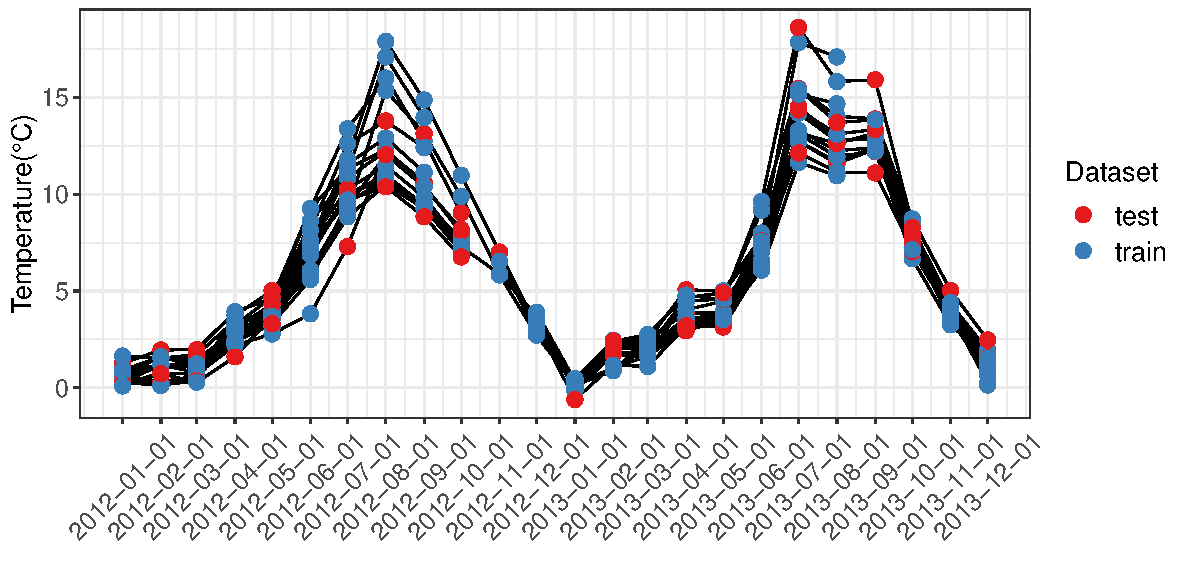
\includegraphics[width=4.5in]{./Figs_Pay/ts.pdf}
  \caption{
  Time series of stream temperatures at multiple locations. Each line represents the time series for a unique observation location. The x-axis represents date, while the y-axis represents the water temperature in C$^{\circ}$. 
Observations (training dataset) are displayed as blue points and the predictions (testing set) are displayed in red. The plot reveals the periodic changes in water temperatures over time at different locations in the stream network.
}
  \label{figure:ts}
\end{figure}


Stream temperature is strongly influenced by topography and climate variables \citep{isaak2017norwest}. The following covariates were available for the observation and prediction locations across all the time points: stream slope, elevation, watershed area \citep{isaak2017norwest}, and air temperature \citep[e.g.][]{bal2014hierarchical}. In addition, we included the first pair of harmonic covariates (Fourier terms) for the time periods  ($\textrm{sin}_t$ and $\textrm{cos}_t$) \citep{forecast}.


\subsection{Visualizing stream network data in space and time}



We begin by extracting the streams from the ssn object so that we can visualise the data in \CRANpkg{ggplot2}. 

\begin{example}
n.df <- SSNbayes::collapse(n)
\end{example}

\noindent The data.frame n.df contains data describing the spatial location of individual stream segments, along with the additive function column. The spatial and space-time data can then be visualised using \CRANpkg{ggplot2} (Fig~\ref{figure:net}). 


\subsection{Fitting spatio-temporal linear models}

The next step is to fit a linear spatio-temporal regression model using the function \texttt{ssnbayes()}. We specify the following linear regression model using the covariates in the observed dataset: 

\begin{equation}
X_{(t)}^{'}\beta = \beta_0 + \beta_1 * \textrm{SLOPE} + \beta_2 * \textrm{elev}  + \beta_3 * \textrm{h2o\_area} + \beta_4 * \textrm{air\_temp}_{(t)} +  \beta_5 * \textrm{sin}_{(t)} + \beta_6 * \textrm{cos}_{(t)}, 
\label{eq:lin}
\end{equation}

\noindent and fit the model to the observed temperature data using the \texttt{ssnbayes()} function. 

\begin{example}
fit_ar <- ssnbayes(formula = temp ~ SLOPE + elev + h2o_area + air_temp + sin + cos, 
                   data = clear,
                   path = path,
                   space_method = list("use_ssn", "Exponential.taildown"),
                   time_method = list("ar", "date"),
                   iter = 3000,
                   warmup = 1500,
                   chains = 3,
                   net = 2, 
                   addfunccol='afvArea',
                   refresh = max(iter/100,1))
\end{example}

\noindent Running this function takes several minutes and the progress of the sampler is shown during the execution. We stored the fitted model within \pkg{SSNdata}, which can be accessed using the code below if the reader wants to skip fitting the model.

\begin{example}
fit_ar <- readRDS(system.file("extdata//fit_ar.rds", package = "SSNdata"))
\end{example}

\noindent The reader is referred to the Appendix for a second reproducible example using simulated data.

In the \texttt{ssnbayes()} function call shown above, the argument \texttt{formula} describes the regression model and is defined in the same way as in other model-fitting functions such as \texttt{lm}. We also pass a data.frame using the \texttt{data} argument, which must contain all of the variables specified in the \texttt{formula} argument. 
This data.frame should be in long format, with one row for each unique observation in space and time, which are also defined using \texttt{locID} and \texttt{pid}. 
%In addition, each spatial location must have the same number of temporal observations collected at the exact same times (even if they are missing). 
In addition, the data set needs to be structured such that each spatial location has the same number of temporal observations.  Such observations can be missing but should be denoted as such via ``NA''.  In such cases, Bayesian imputation is used to obtain a complete data set.
In other words, the data.frame has to contain all the combinations $S$ and $T$. This can be done e.g. using the \texttt{tidyr::complete()} function.

The \texttt{space\_method} argument is a list containing information about the spatial modelling component. The first element specifies whether the topological information is stored in a ssn object or not  (``use\_ssn'' or ``no\_ssn''), while the second list element specifies which spatial correlation model(s) to use. Options include tail-up ("Exponential.tailup", "LinearSill.tailup", "Spherical.tailup"), tail-down ("Exponential.taildown", "LinearSill.taildown", "Spherical.taildown") and 
Euclidean ("Exponential.Euclid") models. 
It is possible to have more than one spatial covariance function per family (tail-up, tail-down and Euclidean distance). For instance: \texttt{space\_method = list('use\_ssn', c("Exponential.tailup", "Spherical.taildown"))}.
However, care should be taken in this case to ensure identifiability of the model.
If the user specifies use\_ssn as the first element and the second element in the list is missing, then an "Exponential.tailup" model will be used by default. When a tail-up covariance function is specified, an additional column containing the additive function values used to compute the spatial weights must also be specified (e.g. \texttt{addfunccol} ='afvArea'). 

    
The argument \texttt{net} specifies the network identifier when multiple networks are found within the same ssn object. 
Much less information is needed to fit traditional Euclidean covariance models and so a ssn object is not needed. Instead, the columns containing the spatial coordinates (e.g. longitude and latitude) must be included as a third element in the list: 
\texttt{space\_method = list("no\_ssn", "Exponential.Euclid", c("lon", "lat"))}. 

The temporal part of the model is defined in a similar fashion using a list \texttt{time\_method = list("method", "date")}. The first element defines the temporal model and options include an autoregressive model, ``ar'', defined in Eq~\ref{eq:case1} or a vector autoregression model, ``var'', defined in Eq~\ref{eq:case2}). The second element is the variable defining the time points in the observation data.frame, which must be a discrete numeric variable. They should also be spaced at regular intervals, as expected in many time series models. 

In \CRANpkg{SSNbayes} the number of chains (\texttt{chains}), iterations (\texttt{iter}), and burn-in samples (\texttt{warmup}) can be specified. 
By default, \texttt{chains} = 3, \texttt{iter} = 3000, \texttt{warmup} = 1500.
Thinning is also possible using the argument \texttt{thin}. Optionally, the \texttt{seed} parameter can be set to ensure reproducibility.

The \CRANpkg{SSNbayes} package depends on \CRANpkg{rstan}, which does not allow missing values in the data. Missing values in the response variable (left hand side element in the formula argument) will be automatically imputed in the \texttt{ssnbayes()} function. 
However, missing values in the covariates (right hand side elements in the formula argument) are not allowed. Instead, they must be imputed by the user before fitting the model. Many options for imputation can be found in \url{https://cran.r-project.org/web/views/MissingData.html}.

The \texttt{ssnbayes()} function shows the progress of the model fit and will be updated based on the number of samples specified using the \texttt{refresh} argument. At every iteration, the inverse of the spatial covariance matrix has to be computed, which takes a substantial amount of time for a 
large number of spatial locations and time points. Fitting this dataset using the \texttt{ssnbayes()} function took approximately 10 minutes on a laptop with an Intel Core i7-8650U CPU @ 1.90GHz and 16 Gb of memory.



\subsection{Exploring results}

The output from \texttt{ssnbayes()} is a \texttt{stanfit} object, which contains information about the fitted model and the MCMC chains for the parameters of interest. It can be summarized and visualized using generic functions such as \texttt{summary()} and \texttt{plot()}, or functions in the \CRANpkg{ggplot2} package. We can also visualize the posterior distributions in the parameters of interest using the \texttt{mcmc\_dens\_overlay()} function from the R package \CRANpkg{bayesplot} \citep{bayesplot}.
The regression coefficients across three chains are shown in Figure~\ref{figure:beta_dens}).

\begin{example}
library('bayesplot')
mcmc_dens_overlay(
  fit_ar,
  pars = paste0("beta[",1:7,"]"),
  facet_args = list(nrow = 1))
\end{example}


Apart from h2o\_area ($\beta_3$), all of the estimated regression coefficients for covariates are substantially different from zero. The bulk of the posterior distribution of the autoregressive parameter ($\phi$) was also far away from zero, suggesting a strong temporal dependence (Figure~\ref{figure:phi_boxplots}). 


\begin{figure}[htbp]
  \centering
   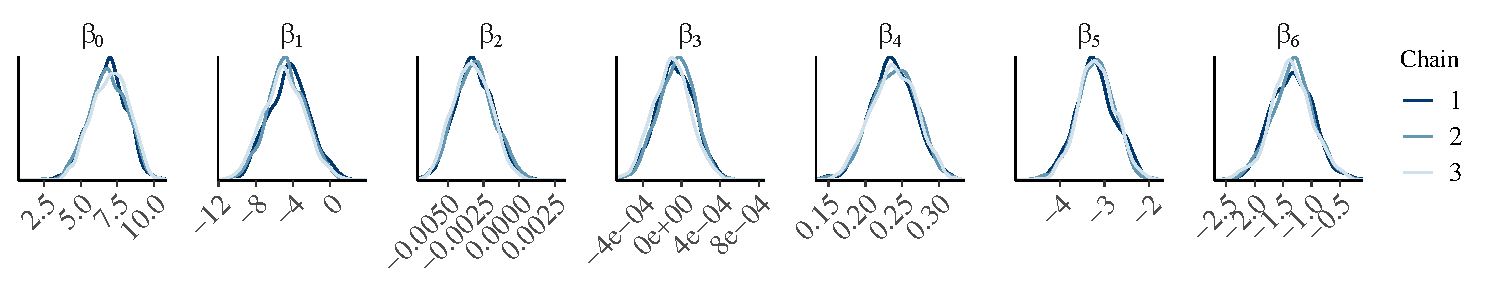
\includegraphics[width=5.6in]{./Figs_Pay/beta_dens.pdf}
  \caption{
  Posterior distributions of the regression coefficients for the linear model with seven covariates, including intercept ($\beta_0$), stream slope ($\beta_1$), elevation ($\beta_2$), watershed area ($\beta_3$), air temperature ($\beta_4$), $\sin$ of day of year ($\beta_5$), and $\cos$ of day of year ($\beta_6$). The distributions are shown for chains 1, 2, and 3, providing insights into the uncertainty and variability of the model coefficients.
  %  Posterior distributions of the regression coefficients [Intercept ($\beta_0$), stream slope ($\beta_1$), elevation ($\beta_2$), watershed area ($\beta_3$), air temperature ($\beta_4$), $\sin$ ($\beta_5$) and $\cos$ ($\beta_6$)] for chains 1, 2, and 3.
  }
  \label{figure:beta_dens}
\end{figure}



\begin{figure}[htbp]
  \centering
   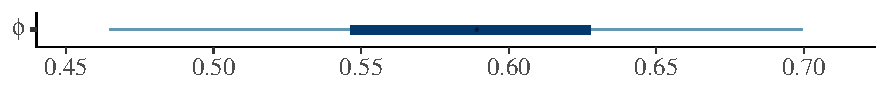
\includegraphics[width=4.0in]{./Figs_Pay/phi_boxplots.pdf}
  \caption{
  Boxplot of the posterior distribution for the autoregression parameter, $\phi$, estimated from the stream temperature time series data. The box represents the interquartile range (IQR). The distribution shows moderate uncertainty in estimating the value of $\phi$.
  }
  \label{figure:phi_boxplots}
\end{figure}


The \texttt{mcmc\_dens\_overlay()} function can also be used to visualise the posterior distributions of the spatial model parameters ($\sigma^2_{TD}$ and $\alpha_{TD}$) and the nugget effect ($\sigma^2_{0}$) (Figure ~\ref{figure:varalphanug}). 

\begin{example}
mcmc_dens_overlay(
  fit_ar,
  pars = c("var_td", "alpha_td", "var_nug"),
  facet_args = list(nrow = 1))
\end{example}

\begin{figure}[htbp]
  \centering
   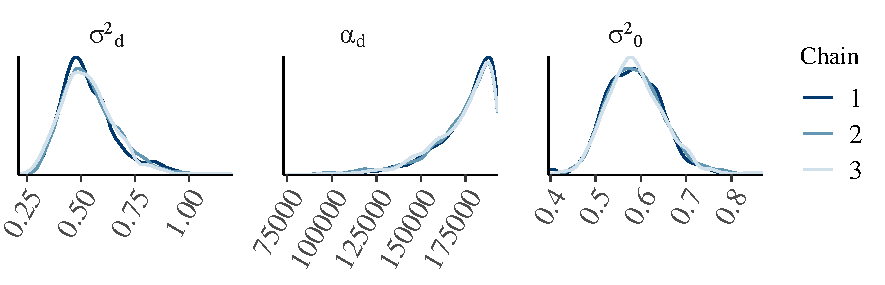
\includegraphics[width=4.0in]{./Figs_Pay/var_alpha_nug.pdf}
  \caption{
  Posterior distributions of the spatial parameters, including the nugget effect ($\sigma^{2}_0$) and the spatial dependence ($\sigma^{2}_d$) in C$^{\circ}$, and the range parameter ($\alpha_d$) in meters.
  }
  \label{figure:varalphanug}
\end{figure}

Notice that the median of the spatial range $\alpha_{TU}$ is approximately 200,000 m, indicating that spatial autocorrelation exists between locations that are less than 200 km apart.





\subsection{Predictions}


Ecological and environmental monitoring on stream networks generally produces data at discrete locations, which represent only a small section of the stream network. However, it is often desirable to make predictions in areas where data have not been collected to create spatially continuous maps \citep{isaak2017norwest}. 
In this section, we illustrate (1) how the model imputes missing values producing predictions, and (2) how to use the fitted model to predict in unsampled locations using a Kriging approach.

As mentioned previously, the \texttt{ssnbayes()} function imputes missing values in the response variable.  
The time series corresponding to the 18 spatial locations are shown in  Fig~\ref{figure:time_series_obs_pred}. 
The model captures the periodic patterns in stream temperatures well, even in locations where most of the observations were missing (e.g. 8 and 12, Fig~\ref{figure:time_series_obs_pred}).
We also compared the predictions produced by the model with the true latent hold-out data (Fig~\ref{figure:true_vs_estimated}).
If the model predictions were perfect we would expect points to fall on the diagonal line. The results suggest that the Bayesian model produces predictions that are similar to the true latent values. Most of the predictions (96\%) were included within the 
95\% highest density interval, showing appropriate coverage of the predictions.  
The root mean square prediction error (RMSPE) between the true temperature values and the predictions was 0.510 \textdegree{}C, which is small considering the magnitude of variation in temperature values.


\begin{figure}[h]
  \centering
   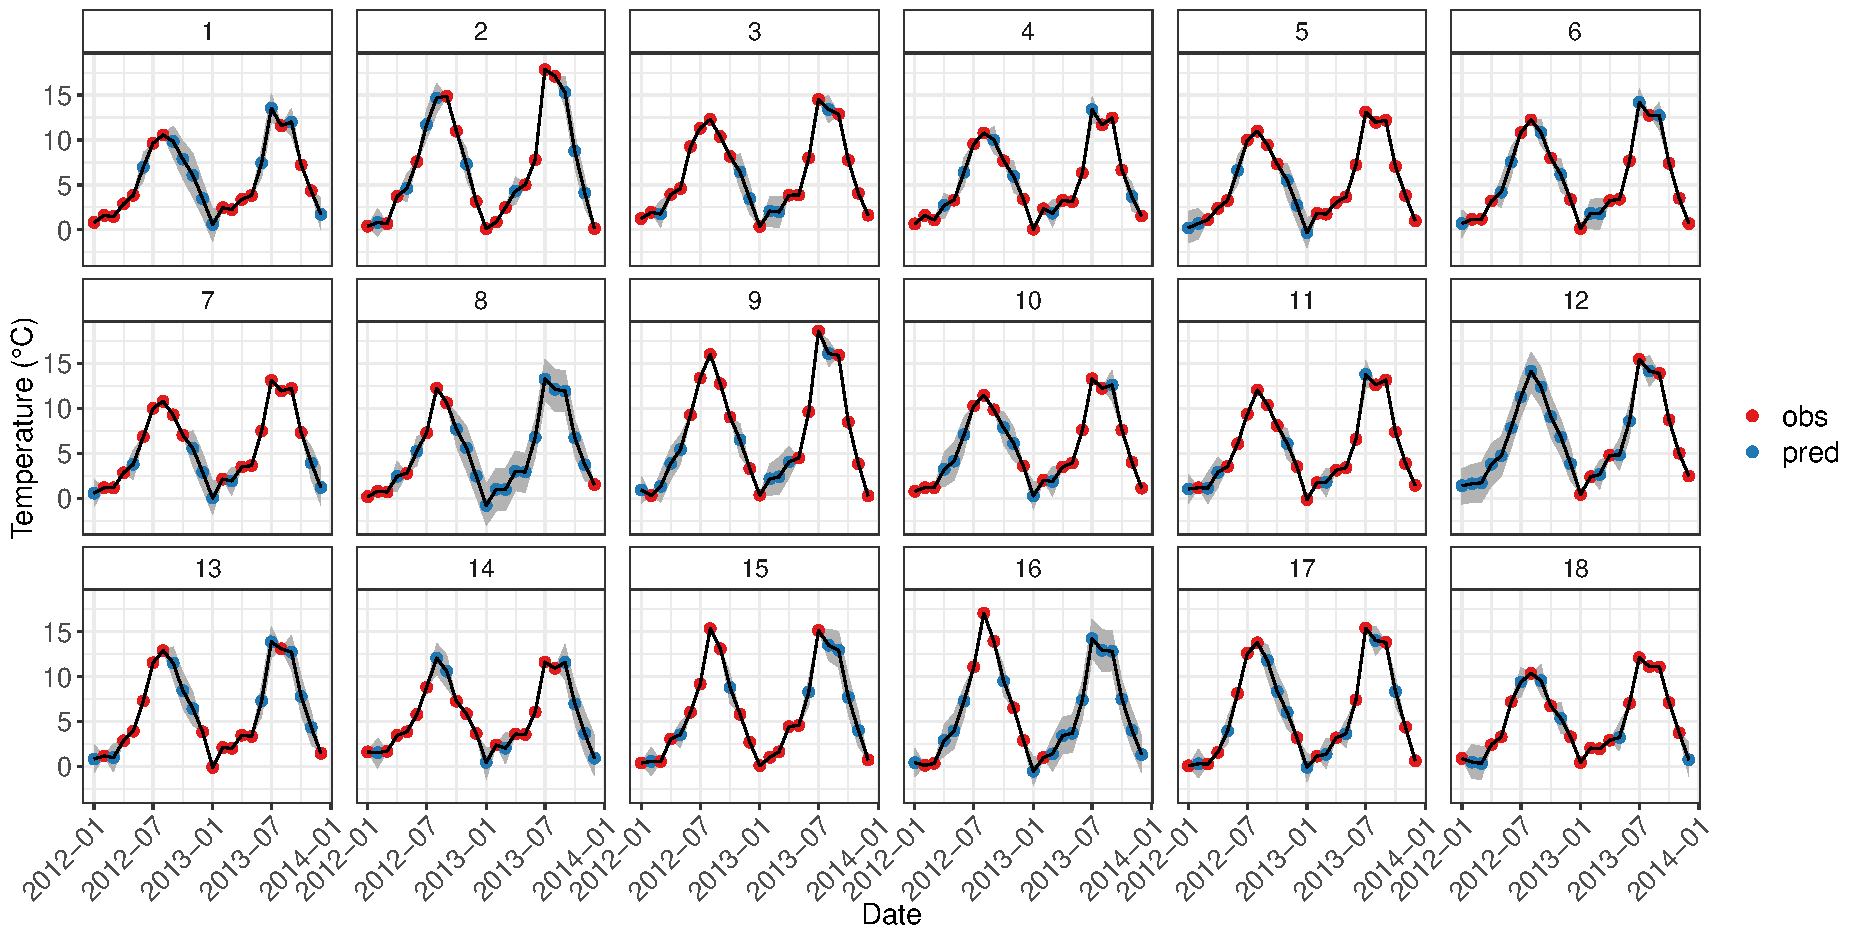
\includegraphics[width=6.0in]{./Figs_Pay/time_series_obs_pred.pdf}
  \caption{
  Time series of stream temperatures at 18 spatial locations. The observed points are represented in red, and the imputed or predicted values are shown in blue. The gray areas represent the 95\% posterior credible intervals, providing an indication of the model's uncertainty.
  }
  \label{figure:time_series_obs_pred}
\end{figure}

\begin{figure}[h]
  \centering
   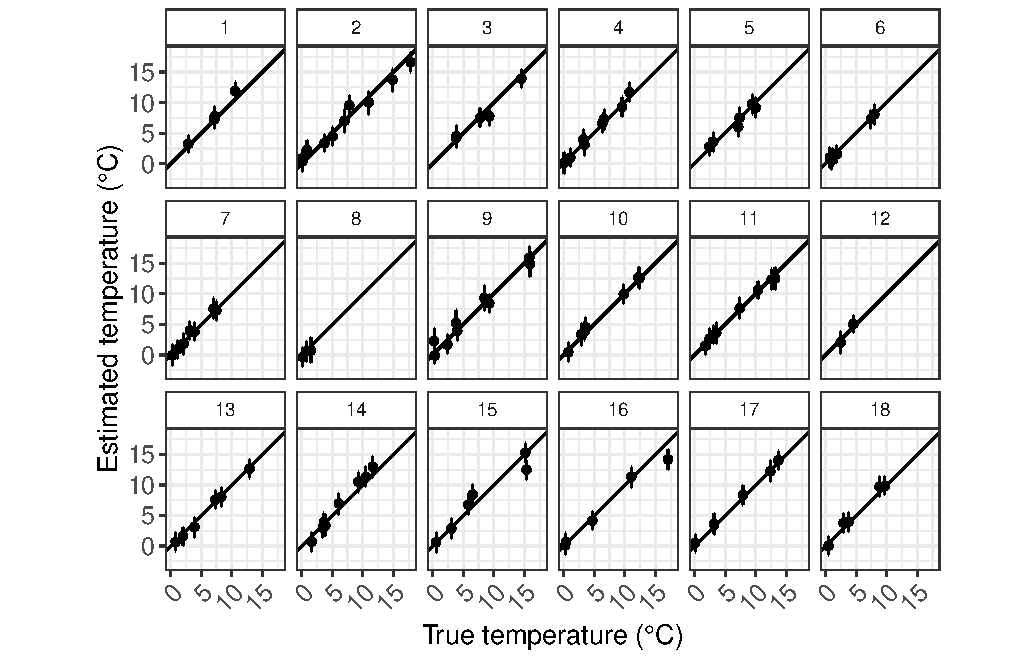
\includegraphics[width=6.0in]{./Figs_Pay/true_vs_estimated.pdf}
  \caption{
  Scatterplot of predicted temperature versus the true latent values at the 18 spatial locations in the test dataset. The x and y axes represent the predicted and true temperature values, respectively. The vertical bars represent the 95\% posterior credible intervals.
  }
  \label{figure:true_vs_estimated}
\end{figure}



Additionally, in our case study, we want to produce temperature predictions at 60 locations generated using a systematic design ($\approx$1km apart). 
The function \texttt{predict()} produces predictions using information contained in the \texttt{stanfit} object obtained from \texttt{ssnbayes()}. The argument  \texttt{nsamples} specifies the number of random samples to select from the posterior distributions and it must be smaller than or equal to the number of iterations  \texttt{iter} specified in \texttt{ssnbayes()}.   


\begin{example}
# reading the prediction data
clear_preds <- readRDS(system.file("extdata/clear_preds.RDS", package = "SSNdata")) 
pred <- predict(path = path,
                      obs_data = clear,
                      stanfit = fit_ar, 
                      pred_data = clear_preds,
                      net = 2,
                      nsamples = 100, # number of samples to use from the posterior 
                      addfunccol = 'afvArea', # additive function values
                      locID_pred = locID_pred,
                      chunk_size = 60)

\end{example}

\noindent The observation and prediction data frames (\texttt{data\_obs}, \texttt{data\_pred}, respectively) must be specified and must contain all of the covariates and the response variable specified in the ``formula'' argument in \texttt{ssnbayes()}. 


Generally, producing subsets of predictions on the stream network is more efficient for big datasets, and can be parallelized. The argument \texttt{chunk\_size} is used to define the size of the subsets. 
For instance, predictions in the case study in \citet{santos2022bayesian} consist of more than 6000 locations. Performing matrix operations with a such large number of sites is not feasible. 
Instead, predictions were run in parallel using \texttt{chunk\_size = 100}.   
\texttt{locID\_pred} also allows the user to define a subset of prediction locations where predictions should be generated, as demonstrated in the example below. Similarly, the argument \texttt{seed} allows the user to set a seed so that the results are reproducible.

Figure ~\ref{figure:preds_ts} shows the predicted time series for the observation and prediction locations. The patterns in the prediction time series captured the seasonality in the observed data well. 
Figure ~\ref{figure:preds_network} visualizes the predictions' posterior mean temperature on the stream network. As expected, higher temperature values are obtained in the main stream channel, compared to predictions in small streams which generally are found at higher elevations. 

\begin{figure}[htbp]
  \centering
   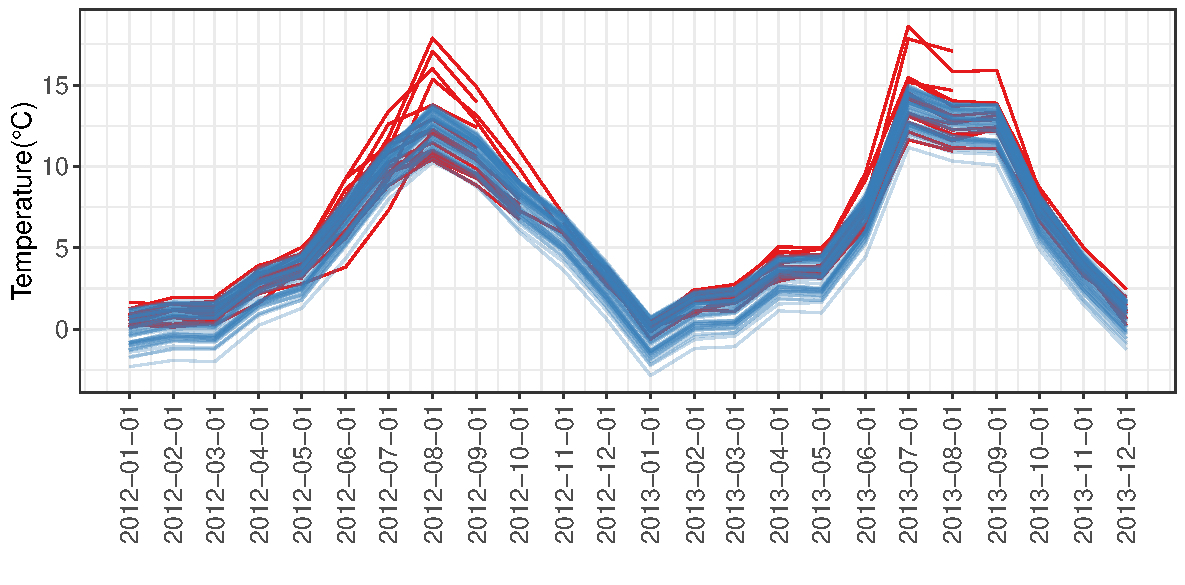
\includegraphics[width=5.0in]{./Figs_Pay/preds_ts.pdf}
  \caption{
  Time series plot comparing predicted (blue lines) and observed (red lines) temperature values over time. }
  \label{figure:preds_ts}
\end{figure}



\begin{figure}[htbp]
  \centering
   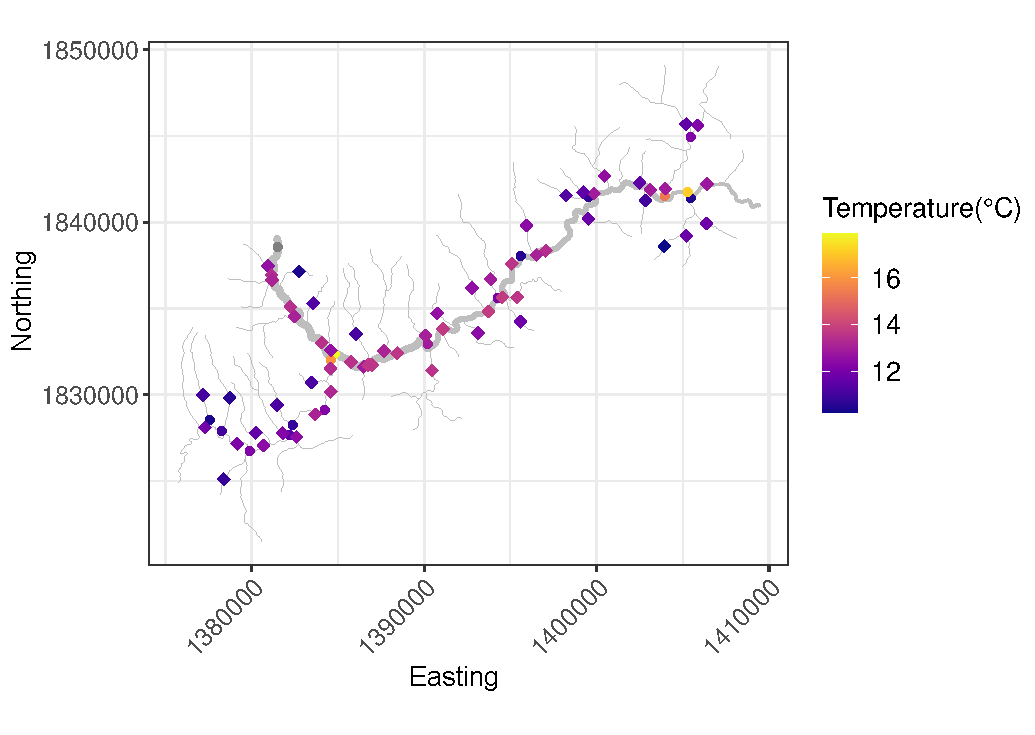
\includegraphics[width=5.75in]{./Figs_Pay/preds_network.pdf}
  \caption{
  Mean daily stream temperature predictions (diamonds) for each of the 60 spatial locations and observations (circles)  in the Clearwater network on August 1st, 2012. 
  %Mean daily stream temperature predictions (diamonds) and observations (circle) in the Clearwater network on 2012-08-01.
  }
  \label{figure:preds_network}
\end{figure}




\subsection*{Network exceedance probability}

One advantage of using Bayesian inference is the ability to easily obtain various probabilistic estimates based on the model posterior predictive samples.
In this example, we use the function \texttt{melt} from the R package \CRANpkg{reshape2} \citep{hadleyreshape2} to generate exceedance probabilities based on a critical thermal threshold of 13 \textdegree{}C for bull trout, a cold-water fish species that is sensitive to increased temperatures.


\begin{example}
ys <- reshape2::melt(pred, id.vars = c('locID0', 'locID', 'date'), value.name ='y')
ys$iter <- gsub("[^0-9.-]", "", ys$variable)
ys$variable <- NULL
# network exceedance probability
limit <- 13
ys$exc <- ifelse(ys$y > limit , 1, 0)
ys <- data.frame(ys) %>% dplyr::group_by(date, locID, locID0) %>% 
  dplyr::summarise(sd = sd(y, na.rm=T),
                   y_pred = mean(y, na.rm=T),
                   prop = mean(exc, na.rm=T)) %>%
  dplyr::arrange(ys, locID)
clear_preds <- clear_preds %>% left_join(ys, by = c('locID', 'date' ))
\end{example}

Figure ~\ref{figure:exc} shows the exceedance probabilities for all 60 prediction locations on two dates, obtained from the posterior predictive distributions. Knowledge about when and where biologically relevant thermal thresholds are likely to be exceeded provides critical information for the management of threatened and endangered freshwater species \citep{isaak2016slow}.   


\begin{figure}[htbp]
  \centering
   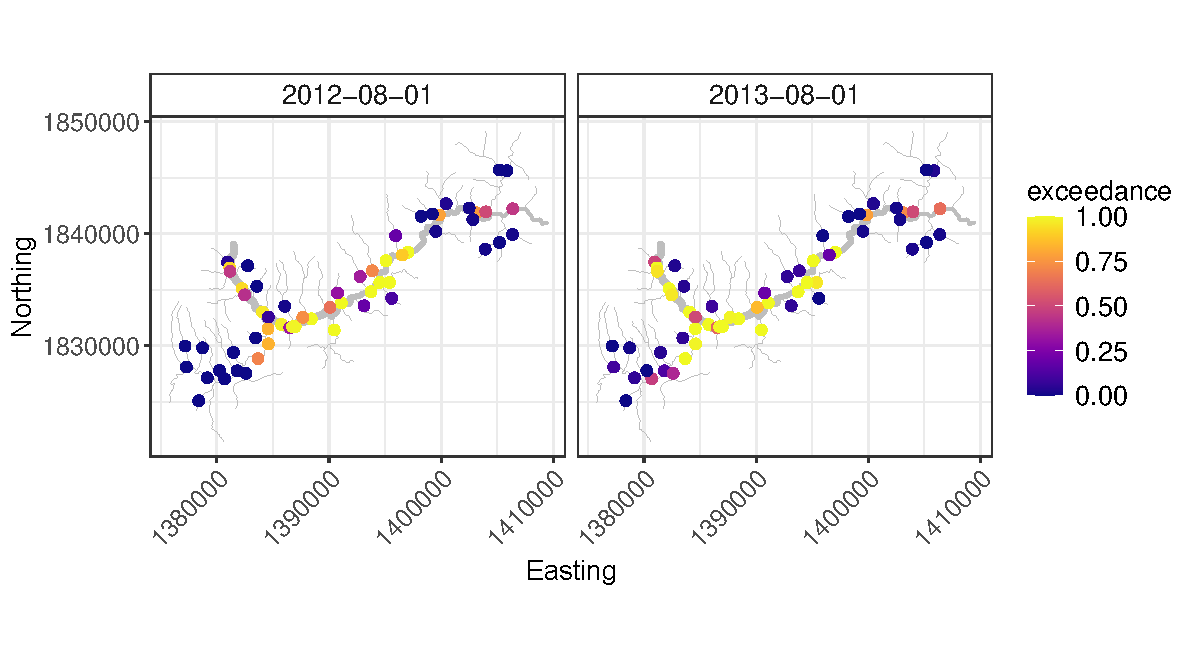
\includegraphics[width=6.0in]{./Figs_Pay/exc.pdf}
  \caption{
  Probabilities that the mean stream temperature will exceed the 13 \textdegree{}C threshold on August 1, 2012, and August 1, 2013, respectively across the 60 prediction locations in the Clearwater network.
  %Probabilities that the mean stream temperature will exceed the 13 \textdegree{}C threshold on 2012-08-01 and 2013-08-01.
  }
  \label{figure:exc}
\end{figure}




\subsection*{Other useful functions}
Users often want to extract distance matrices and spatial weights so that they can be analysed and/or visualised in other R packages or external software e.g. \citet{McGuire14}. The \texttt{dist\_weight\_mat()} and \texttt{dist\_weight\_mat\_preds()} produce a list of distance and weight matrices with the following elements:

\begin{enumerate}
    \item e: Euclidean distance matrix containing the distances between locations
    \item D: Downstream distance.
    \item H: Total stream distance.
    \item w.matrix: spatial weights for flow connected locations. This matrix is used in the tail-up models. 
    \item flow.con.mat: flow connected matrix. Indicates whether two locations in the network are connected by flow.
\end{enumerate}

The \texttt{dist\_weight\_mat()} function produces matrices of the distances and weights between observation locations, with dimensions equal to the number of observation locations ($n_o \times n_o$). The \texttt{dist\_weight\_mat\_preds()} function produces the same information for observed and prediction locations, with  $n_o n_p \times n_o n_p$ dimensions.
Details and detailed descriptions of the computation of these matrices can be found in \citet{peterson2010mixed}, \citet{hoef2014ssn}, and \citet{santos2022bayesian}.







\section{Discussion and conclusions}
\label{sec:dis}

The growing popularity of stream sensor arrays, in which repeated observations are taken at multiple sites, requires models capable of accounting for spatial and temporal autocorrelation in stream network data.    
However, there are only a limited number of computational methods and software packages designed to account for the unique spatial dependence found in stream data (e.g. the R packages \CRANpkg{SSN}, \CRANpkg{SSN2}  and \CRANpkg{smnet}). 
The package described in the present paper extends the models implemented in \CRANpkg{SSN} by accounting for temporal dependence using Bayesian inference, which offers several benefits.
Enhanced features from this package and other benefits from the use of a Bayesian framework include the computation of probabilistic estimates and network exceedance probabilities, the ability to incorporate prior information, and the estimation of the proportion of degraded habitat.   


We tested the performance of \CRANpkg{SSNbayes} in multiple scenarios with simulated and real data and found that the parameters are well estimated and the predictions are accurate in terms of RMSPE. 
We also validated the results from a wide range of spatial model combinations to those obtained using \CRANpkg{SSN} based on simulated data.  
Spatial and spatio-temporal models tend to be slow to fit and computationally intensive, which becomes more challenging within a Bayesian modelling framework. This can become computationally prohibitive when the number of spatial locations is large because the spatial covariance matrix must be iteratively inverted. We are currently exploring alternative methods (such as variational Bayes) to be implemented within \CRANpkg{SSNbayes}.

Future implementations will incorporate other modelling variations.
Two of them are: (I) expressing $\phi_s$ as a linear combination of covariates such as elevation and watershed (an extension of Case 2), and (II)
using a 2-Nearest Neighbours (2-NN) method, where the off-diagonal elements of $\pmb{\Phi}$ are different from zero in the two closest, allowing temporal dependence to be established between neighbouring spatial locations connected by flow \citep{santos2022bayesian}. 
However, other space-time covariance structures could also be implemented for stream network data, which allow more modelling flexibility. For example, this implementation is based on a vector autoregression structure, but other models such as moving averages and ARIMA could also be considered. In addition, we currently assume that the response variable is normally distributed, but other regression models could be implemented by modifying the likelihood function in \texttt{ssnbayes()}. 
We are also actively working on the development and implementation of models for anomaly detection in stream data \citep{santos2023unsupervised}.
The \CRANpkg{SSNbayes} package is under constant development and new features and model implementations are on their way. 





\section*{Acknowledgement}

This research was supported by the Australian Research Council (ARC) Linkage Project ``Revolutionising water-quality monitoring in the information age'' (ID: LP180101151) and the Centre of Excellence for Mathematical and Statistical Frontiers (ACEMS). 
JMM was supported by an Australian Research Council Discovery Project (DP200101263).
We thank Dona Horan for the creation of the spatial stream network (.ssn) object.
Data analysis and computations were undertaken using the packages \CRANpkg{rstan} \citep{rstan}. Data visualizations were made with the packages \CRANpkg{ggplot2} \citep{ggplot2} and \CRANpkg{bayesplot} \citep{bayesplot}. 
%\textsf{R}

\appendix
\section*{Appendix}
\label{sec:appndx} 





In this appendix, we illustrate the fit of a spatio-temporal stream network model within the Bayesian framework with \CRANpkg{SSNbayes} using a simulated example. These results can be reproduced using the Kaggle notebook \url{https://www.kaggle.com/code/edsans/ssnbayes-simulated}. Several R packages must be installed to successfully reproduce the simulation described in this section. Installing the \CRANpkg{rstan} can be tricky because you need to configure your R installation to be able to compile C++ code. If you have not used the \CRANpkg{rstan} before, please see https://github.com/stan-dev/rstan/wiki/RStan-Getting-Started for easy-to-follow instructions about how to install the package.




\subsection*{Using simulated data}


We generated some spatial data with the \CRANpkg{SSN} package using a systematic design for the locations of the observations and predictions. Note that the \CRANpkg{SSN} package has been archived on CRAN. 

\begin{example}
## Load the packages. Note that these packages can be installed 
## using the install.packages() function
library('tidyverse')
library('Rcpp')
library('StanHeaders')
library('rstan')
library('abind')
library('SSN')
library('SSN2')
library('bayesplot')
library('lubridate')
library('viridis')
library('ggrepel')
library('devtools')
library('RColorBrewer')
if(!require('SSNbayes')) install.packages("SSNbayes", dependencies = T)
library('SSNbayes')
\end{example}


\begin{example}
## Set some useful options for modelling
rstan_options(auto_write = TRUE) # avoid recompilation
options(mc.cores = parallel::detectCores())
RNGkind(sample.kind = "Rounding")

## Set the seed for reproducibility
seed <- 202008
set.seed(seed)

## Set the path for the SpatialStreamNetwork object created in the next step
path <- "./sim.ssn"

## If it does not already exist, create a SpatialStreamNetworkObject
## with 150 stream segments (edges). Use a systematic design to generate
## observed and prediction locations on the network spaced
## approximately 3 and 0.3 units apart, respectively.
if(file.exists(path)){
  ssn <- importSSN(path, "preds")
}  else{ssn <- createSSN(n = c(150),  # 150 edges
               obsDesign = systematicDesign(spacing=3),
               predDesign = systematicDesign(spacing=0.3),
               importToR = TRUE,
               path = path, # path where the sns object is saved
               treeFunction = iterativeTreeLayout)}
\end{example}

This produces a SpatialStreamNetwork object with 50 observation locations, which is our training dataset. We also generated 499 prediction locations for testing. 

\begin{example}
## Plot the edges and observed locations in the SpatialStreamNetwork object
plot(ssn, lwdLineCol = "addfunccol",  lwdLineEx = 8,
     lineCol = 4,  col = 1,  pch = 16,  xlab = "x-coordinate",  ylab = "y-coordinate")
\end{example}

\begin{example}
## Add the prediction locations
plot(ssn, PredPointsID = "preds", add = T, pch = 16, col = "#E41A1C")
\end{example}

Consider a response variable such as stream temperature. 
The aim is to predict this response variable in the testing dataset borrowing information from other measurements across space and time and using covariates such as air temperature. Predictions can be made at a subset of locations or across all prediction locations on the whole network.

Distances within and between observation and prediction locations must be generated before model fitting. 

\begin{example}
## Create stream distance matrices
createDistMat(ssn, predpts = 'preds',o.write=TRUE, amongpreds = T)
\end{example}

We then need to simulate some data using some covariates, regression coefficients and a covariance structure.

\begin{example}
## Extract the data.frames for the observed and prediction location data
rawDFobs <- getSSNdata.frame(ssn, Name = "Obs")
rawDFpred <- getSSNdata.frame(ssn, Name = "preds")

## Extract the geographic coordinates from the SpatialStreamNetwork
## object and add to data.frames
obs_data_coord <- data.frame(ssn@obspoints@SSNPoints[[1]]@point.coords)
obs_data_coord$pid<- as.numeric(rownames(obs_data_coord))
rawDFobs<- rawDFobs %>% left_join(obs_data_coord, by = c("pid"),
                                  keep = FALSE)
rawDFobs$point <- "Obs" ## Create label for observed points

pred_data_coord <- data.frame(ssn@predpoints@SSNPoints[[1]]@point.coords)
pred_data_coord$pid<- as.numeric(rownames(pred_data_coord))
rawDFpred<- rawDFpred %>% left_join(pred_data_coord, by = "pid",
                                    keep = FALSE)
rawDFpred$point <- "pred" ## Create label for prediction points

## Generate 3 continuous covariates at observed and prediction locations
set.seed(seed)
rawDFpred[,"X1"] <- rnorm(length(rawDFpred[,1]))
rawDFpred[,"X2"] <- rnorm(length(rawDFpred[,1]))
rawDFpred[,"X3"] <- rnorm(length(rawDFpred[,1]))

rawDFobs[,"X1"] <- rnorm(length(rawDFobs[,1]))
rawDFobs[,"X2"] <- rnorm(length(rawDFobs[,1]))
rawDFobs[,"X3"] <- rnorm(length(rawDFobs[,1]))

## Ensure the rownames still match the pid values used in the
## SpatialStreamNetwork object
rownames(rawDFobs)<- as.character(rawDFobs$pid)
rownames(rawDFpred)<- as.character(rawDFpred$pid)

## Put the new covariates back in the SpatialStreamNetwork object
ssn <- putSSNdata.frame(rawDFobs,ssn, Name = 'Obs')
ssn <- putSSNdata.frame(rawDFpred, ssn , Name = 'preds')

## Simulate the response variable at observed and prediction locations
set.seed(seed)
sim.out <- SimulateOnSSN(ssn.object = ssn,
                          ObsSimDF = rawDFobs, ## observed data.frame
                          PredSimDF = rawDFpred, ## prediction data.frame
                          PredID = "preds", ## name of prediction dataset
                          formula = ~ X1 + X2 + X3,
                          coefficients = c(10, 1, 0, -1), ## regression coefficients
                          CorModels = c("Exponential.taildown"), ## covariance model
                          use.nugget = TRUE, ## include nugget effect
                          CorParms = c(3, 10, .1)) ## covariance parameters

## Extract the SpatialStreamNetwork object from the list returned by
## SimulateOnSSN and extract the observed and prediction site
## data.frames. Notice the new column Sim_Values in the data.frames
sim.ssn <- sim.out$ssn.object
simDFobs <- getSSNdata.frame(sim.ssn,"Obs")
simDFpreds <- getSSNdata.frame(sim.ssn, "preds")
summary(simDFobs)
\end{example}

The SpatialStreamNetwork object we created only contains one simulated response for each observation and prediction location and we can fit a spatial statistical model to the simulated data using the \texttt{glmssn} function in the \CRANpkg{SSN} package. 

\begin{example}
## Fit a spatial stream network model using the Exponential tail-down function
glmssn.out <- glmssn(Sim_Values ~ X1 + X2 + X3, sim.ssn,
                     CorModels = "Exponential.taildown")
summary(glmssn.out)
\end{example}

In order to fit a space-time model using the \CRANpkg{SSNbayes} package, we need repeated measurements at each location. We now need to generate some time series with AR(1) error structure:

\begin{example}
## Create a data.frame containing training and test data.
df_obs <- getSSNdata.frame(sim.ssn, "Obs") ## Extract observed dataset
df_obs$dataset <- 'train' ## Create new column 'dataset' and set to 'train'
df_pred <- getSSNdata.frame(sim.ssn, "preds") ## Extract prediction dataset
df_pred$dataset <- 'test' ## Create new column 'dataset' and set to 'test'

## Expand data.frames to include 10 days per location
t <- 10 # days
df_obs <- do.call("rbind", replicate(t, df_obs, simplify = FALSE))# replicating the df
df_obs$date <- rep(1:t, each = (nrow(df_obs)/t)) # Set date variable

df_pred <- do.call("rbind", replicate(t, df_pred, simplify = FALSE))# replicating the df
df_pred$date <- rep(1:t, each = (nrow(df_pred)/t)) # Set date variable
 
## Create a copy of the pid value used in the SpatialStreamNetwork
## object and create a new pid value for use in SSNbayes
## package. Values must be consequtively ordered from 1 to the number
## of rows in the data.frame
df_obs <- df_obs %>% mutate(pid.ssn = pid,
                            pid = rep(1:nrow(.)))
df_pred <- df_pred %>% mutate(pid.ssn = pid,
                            pid = rep(1:nrow(.)))

## Combine the training and testing datasets
df <- rbind(df_obs, df_pred) 
df$dataset <- factor(df$dataset, levels = c('train', 'test'))

## Construct and initialize an autocorrelation structure of order 1
set.seed(seed)
phi <- 0.8 ## lag 1 autocorrelation value
ar1 <- corAR1(form = ~ unique(df$date), value = phi) # can also use corExp function
AR1 <- Initialize(ar1, data = data.frame(unique(df$date)))

## Create a vector of AR1 errors for each date and expand to all all locations
epsilon <- t(chol(corMatrix(AR1))) %*% rnorm(length(unique(df$date)), 0, 3)   #NB AR1 error
epsilon <- rep(epsilon, each = length(unique(df$locID)) ) +
  rnorm(length(epsilon)*length(unique(df$locID)), 0, 0.25) # for all the locations
epsilon_df <- data.frame(date = rep(unique(df$date), each = length(unique(df$locID))),
                         locID = rep(unique(df$locID), times = length(unique(df$date))),
                         epsilon = epsilon)
df <- df %>% left_join(epsilon_df, by = c('date' = 'date', 'locID' = 'locID'))

## Create a new simulated response variable, y, with errors added
df$y <- df$Sim_Values + df$epsilon 
\end{example}


We can visualize the time series of the new simulated response at the observed and predicted locations over time:
\begin{example}
## Create line plots of response over time for training and test datasets
ggplot(df) +
  geom_line(aes(x = date, y = y, group = locID, col = dataset), alpha = 0.4) +
  ylab("Simulated Temperature (\u00B0C)")+
  facet_wrap(~dataset)+
  theme_bw()
\end{example}

Figure~\ref{figure:1time_series} shows the stream temperature time series in the observations and predictions datasets.

\begin{figure}[htbp]
  \centering
   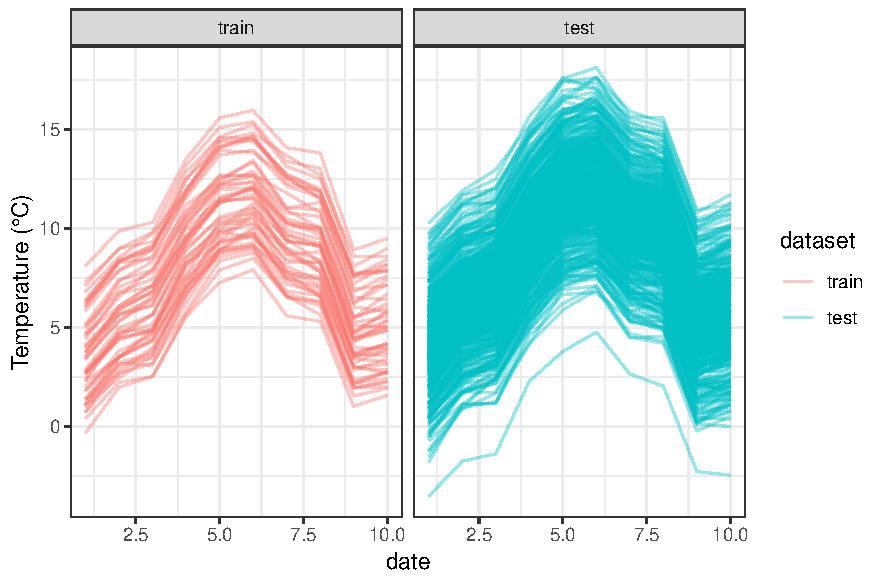
\includegraphics[width=4.0in]{./Figs/1time_series.pdf}
  \caption{Evolution of the stream temperature time series in the observations and predictions datasets. Each time series represent a spatial location.}
  \label{figure:1time_series}
\end{figure}



\begin{example}
## Split the training and testing datasets. Ensure that date is numeric.
df <- df %>% dplyr::select(locID, pid, date, y, everything())
obs_data <- df[df$dataset == 'train',]
pred_data <- df[df$dataset == 'test',]
# NB: the order in this data.fame MUST be: spatial locations (1 to S) at time t=1, 
# then locations (1 to S) at t=2 and so on.

\end{example}


The first prediction option in \CRANpkg{SSNbayes} is to generate predictions for locations in the observed dataset with missing data. To demonstrate, let us set approximately 30\% of the observations per date to missing, make predictions, and assess how well we retrieve the actual temperature values. 

\begin{example}
# Randomly select observations by date
set.seed(seed)
points <- length(unique(obs_data$pid))
locs <- obs_data %>% dplyr::group_by(date) %>%
   pull(pid) %>%
  sample(., round(points * 0.3), replace = F)  %>% sort()

## Create a backup for the response before setting randomly selected
## measurements to NA
obs_data$y_backup <- obs_data$y
obs_data[obs_data$pid %in% locs,]$y <- NA

\end{example}


Let us visualize the network with the time series of observed temperature values.
First we use the \textsf{collapse()} function to extract the network structure from the the SpatialStreamNetwork object. 
The facets (1-10) represent the date and there are a total of 150 missing observations (gray dots) which are observations that we set to missing to assess the model predictive accuracy.

\begin{example}
## Extract stream (edge) network structure, including the additive function value
nets <- SSNbayes::collapse(ssn, par = 'addfunccol')

## Create additive function value categories for plotting
## Create additive function value categories for plotting
nets$afv_cat <- cut(nets$addfunccol,
                                 breaks = seq(min(nets$addfunccol),
                                              max(nets$addfunccol),
                                              length.out=6),
                                 labels = 1:5,
                                 include.lowest = T)

## Plot simulated temperature, by date, with line width proportional to afv_cat
ggplot(nets) +
    geom_path(aes(X1, X2, group = slot, size = afv_cat), lineend = 'round',
              linejoin = 'round', col = 'lightblue')+
    geom_point(data = dplyr::filter(obs_data, date %in% 1:10),
               aes(x = coords.x1, y = coords.x2, col = y, shape = point),
               size = 1)+
  scale_size_manual(values = seq(0.2,2,length.out = 5))+
  facet_wrap(~date, nrow = 2)+
  scale_color_viridis(option = 'C')+
  scale_shape_manual(values = c(16,15))+
  xlab("x-coordinate") +
  ylab("y-coordinate")+
  theme_bw()

\end{example}


\begin{figure}[htbp]
  \centering
   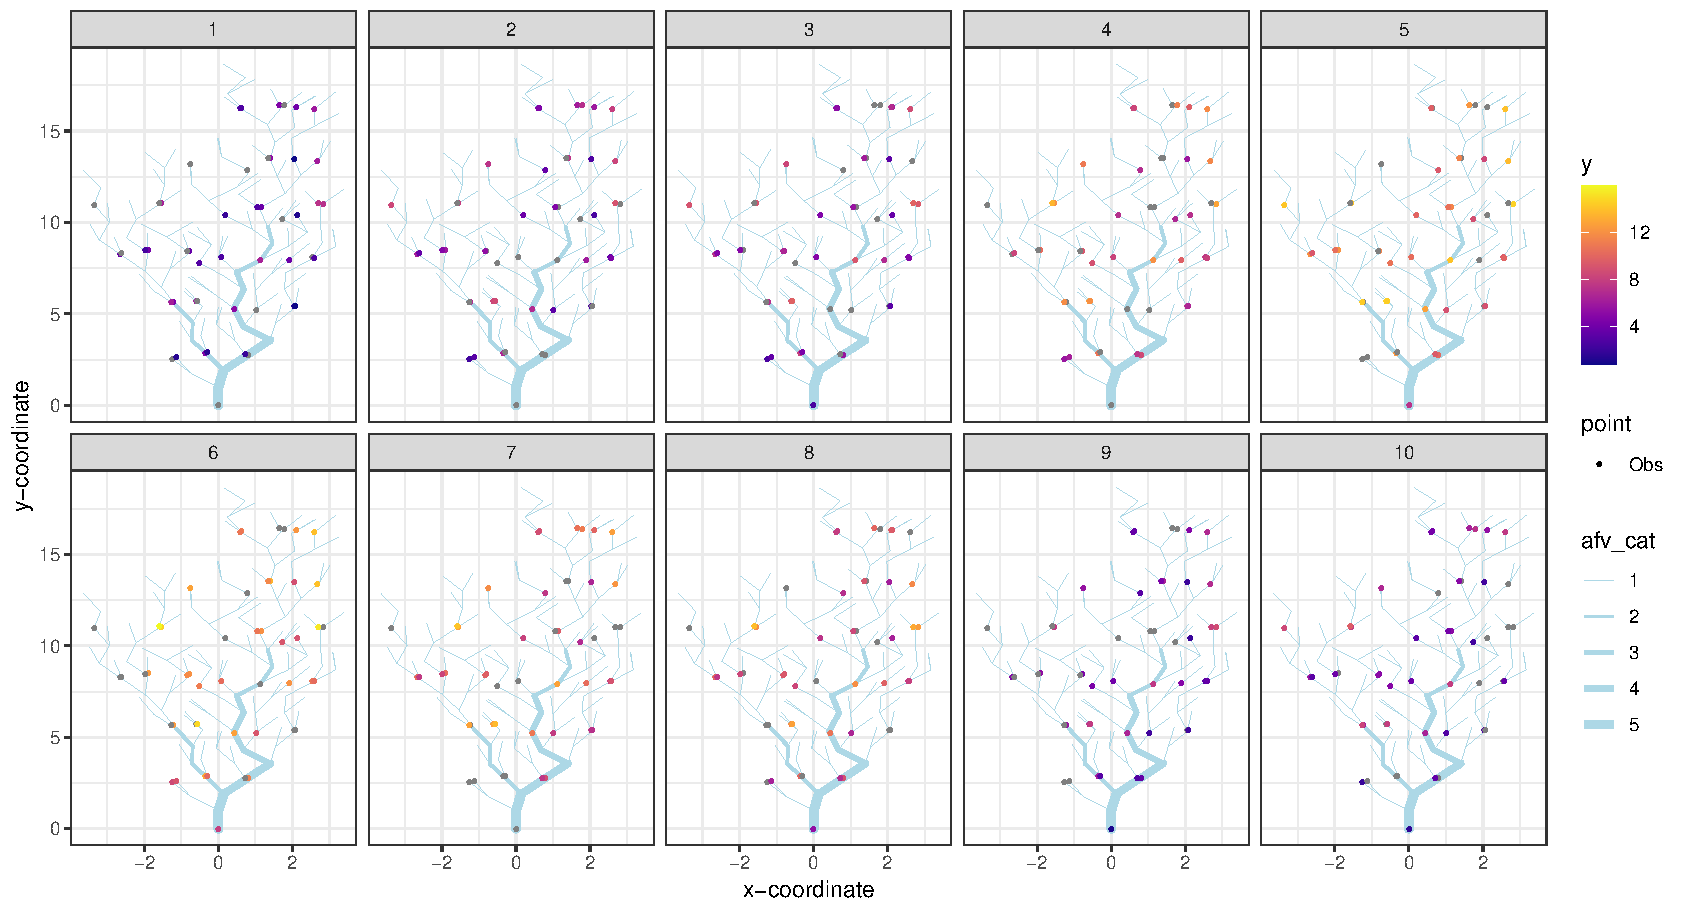
\includegraphics[width=6.0in]{./Figs/2network_time_obs.pdf}
  \caption{Evolution of the stream temperature time series in the observation dataset across ten time points.}
  \label{figure:2network_time_obs}
\end{figure}


\pagebreak

We then fit a Bayesian space-time model, with a tail-down covariance model and an AR(1) error structure using the \texttt{ssnbayes()} function.
Fitting the model took about 15 minutes on a laptop (i7 @1.80 GHz and 16GB RAM).


\begin{example}
## Fit a Bayesian space-time model
fit_td <- ssnbayes(formula = y ~ X1 + X2 + X3,
                   data = obs_data,
                   path = path,
                   time_method = list("ar", "date"), # temporal model to use
                   space_method = list('use_ssn', c("Exponential.taildown")), # spatial model
                   iter = 4000,
                   warmup = 2000,
                   chains = 3,
                   addfunccol = 'addfunccol',
                   loglik = T)

## Create a copy of the model fit and set class so that we can take
## advantage of plotting functions for stanfit objects
fits <- fit_td
class(fits) <- c("stanfit")

## Extract summaries of the posterior distributions for the parameter
## estimates and the predictions.
stats_td <- summary(fits)
stats_td <- stats_td$summary
\end{example}

One of the main benefits of this Bayesian approach is that the model produces probabilistic estimates.
Figures ~\ref{figure:3densities_pars} and  ~\ref{figure:3densities_beta} show the posterior distributions of the four parameters in the spatio-temporal model ($\sigma^2_{TU}$, $\sigma^2_{0}$, $\alpha$ and $\phi$ ) and the regression coefficients (intercept and slopes).  
The trace plots for of these parameters can be found in the Appendix \ref{sec:others}.



\begin{example}
## Create plots of the posterior distribution of the 3 regression
## coefficients
mcmc_dens_overlay(
  fits, #
  pars = paste0("beta[",1:3,"]"),
  facet_args = list(nrow = 1))

## Plot the posterior distribution of phi
mcmc_intervals(
  fits,
  pars = paste0("phi"),
  point_size = .1,
  prob_outer = 0.95
)

## Plot the posterior distribution for the nugget effect, partial sill.
## and range parameters in the tail-down model
mcmc_dens_overlay(
  fits,
  pars = c(
    "var_td",
    "alpha_td",
    "var_nug"),
  facet_args = list(nrow = 1)
)
\end{example}


\begin{figure}[htbp]
  \centering
   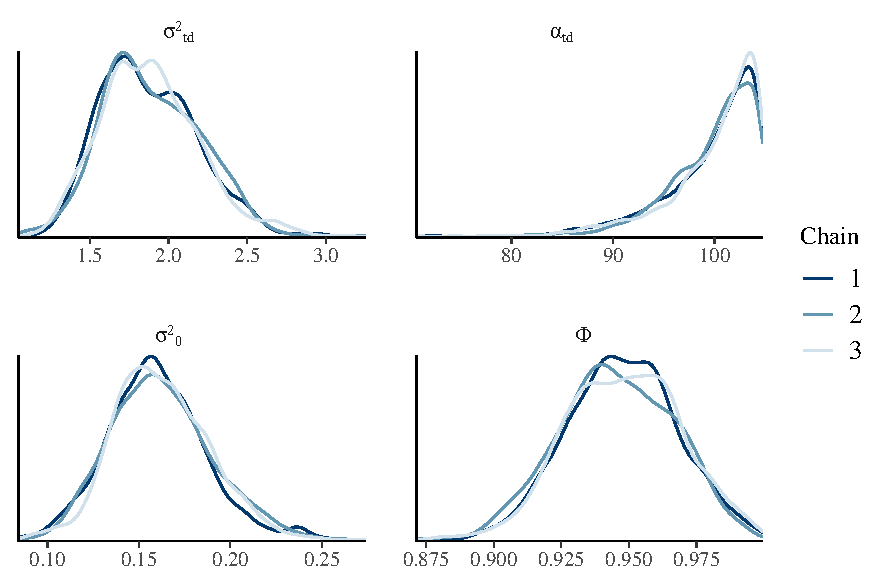
\includegraphics[width=5.0in]{./Figs/3densities_pars.pdf}
  \caption{Posterior densities of the partial sill ($\sigma^2_{TU}$), nugget effect ($\sigma^2_{0}$), range ($\alpha$) and temporal autocorrelation $\phi$ parameters.
  These parameters are crucial for understanding the spatial and temporal variability in the simulated stream network dataset.
  }
  \label{figure:3densities_pars}
\end{figure}



\begin{figure}[htbp]
  \centering
   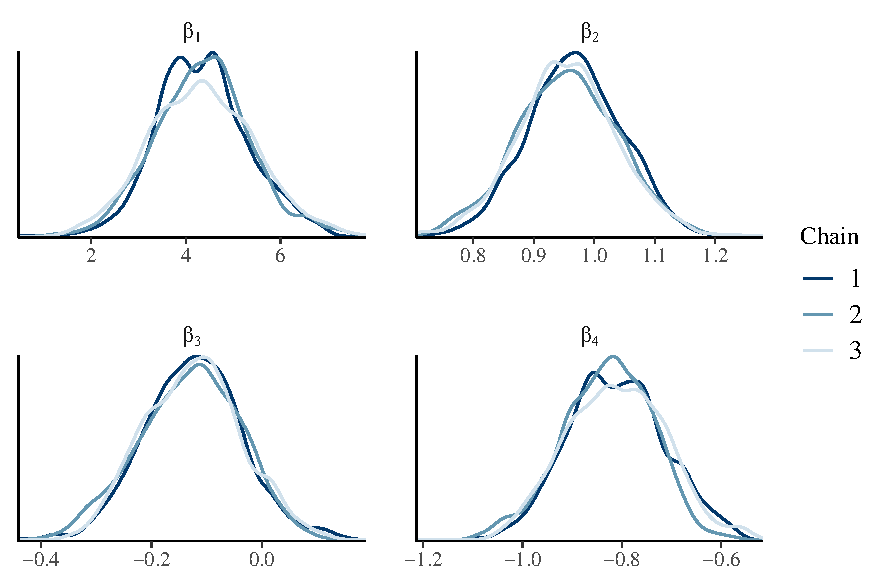
\includegraphics[width=5.0in]{./Figs/3densities_beta.pdf}
  \caption{Posterior densities of the regression coefficients ($\beta$) for the intercept ($\beta_1$) and the three covariates X1, X2, and X3 ($\beta_2$, $\beta_3$, and $\beta_4$, respectively). }
  \label{figure:3densities_beta}
\end{figure}


We then assess how accurate the predictions of the missing temperature values are compared to the true held out values.

\begin{example}
## Create a data.frame containing summaries of the posterior predictive
## distributions and the true values
ypred <- data.frame(stats_td[grep("y\\[", row.names(stats_td)),])
ypred$ytrue <- obs_data$y_backup #
ypred$date <- rep(1:t, each = nrow(obs_data)/t)
ypred$dataset <- ifelse(ypred$sd == 0, 'obs', 'pred')
ypred$td_exp <- ypred$mean

## Create a plot of the predicted versus true values with 95% highest
## density interval
 filter(ypred, dataset == 'pred') %>% ggplot() +
     geom_errorbar(data = ypred, aes(x=ytrue, ymin=X97.5., ymax=X2.5.),
                   col = 2, width=0.5, size=0.5, alpha = 0.75) +
  geom_point(aes(x = ytrue , y = td_exp), col = 2)+
  geom_abline(intercept = 0, slope = 1)+
  facet_wrap(~date, nrow = 2) +  coord_fixed() +
     xlab('y true') + ylab('y estimated') +  theme_bw()

## Calculate the root mean square error (RMSE) between the true and
## predicted values
rmse <- sqrt(mean(((ypred$ytrue) - ypred$td_exp)^2))
rmse

# Calculate the 95% prediction coverage. Ideally, this should be close to 0.95. 
ypred$cov <- ifelse(ypred$ytrue > ypred$X2.5. & ypred$ytrue<ypred$X97.5,1,0)
filter(ypred, dataset == 'pred') %>%
  group_by(dataset) %>%
  dplyr::summarize(mean(cov))


\end{example}

In Figure ~\ref{figure:4y_true_vs_pred}, we have plotted the means of the imputed values (with a 95\% prediction interval) against the true values of the missing data.  As can be seen, the means of each imputed value largely agree with the true value, with most prediction intervals (96\%) containing the true value.
The RMSE of the predicted temperature ($y$) is 0.245 which is small compared to the magnitude of $y$ (Mean = 7.621 and standard deviation = 3.489 degrees). 
Figure ~\ref{figure:3densities_y} shows the posterior densities of the predicted temperature ($y$) for 8 measurements in the testing set.  


\begin{figure}[htbp]
  \centering
   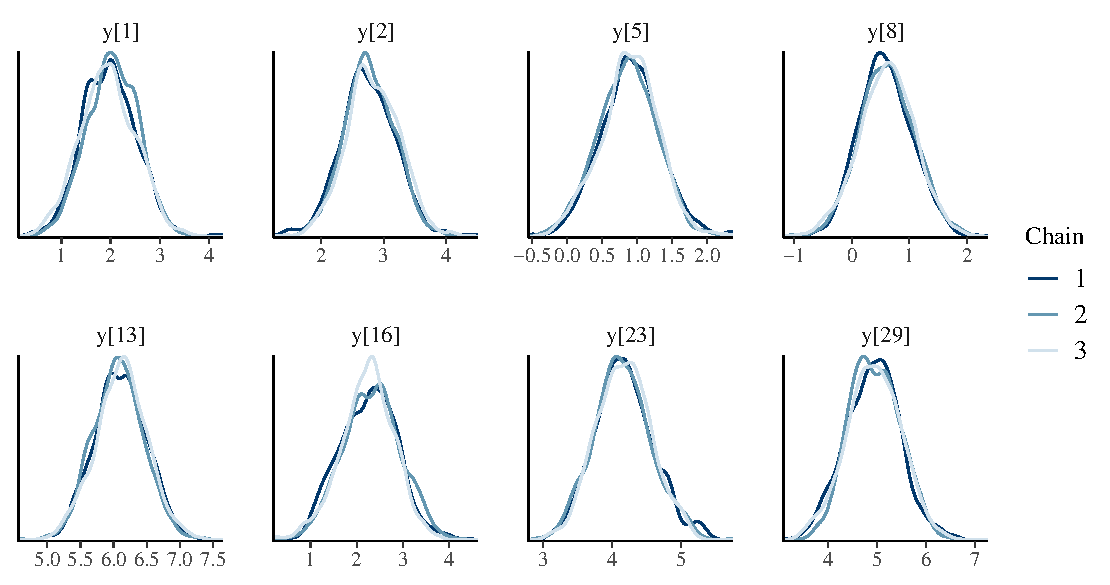
\includegraphics[width=5.0in]{./Figs/3densities_y.pdf}
  \caption{Posterior densities for 8 temperature predictions ($y$). }
  \label{figure:3densities_y}
\end{figure}

\begin{figure}[htbp]
  \centering
   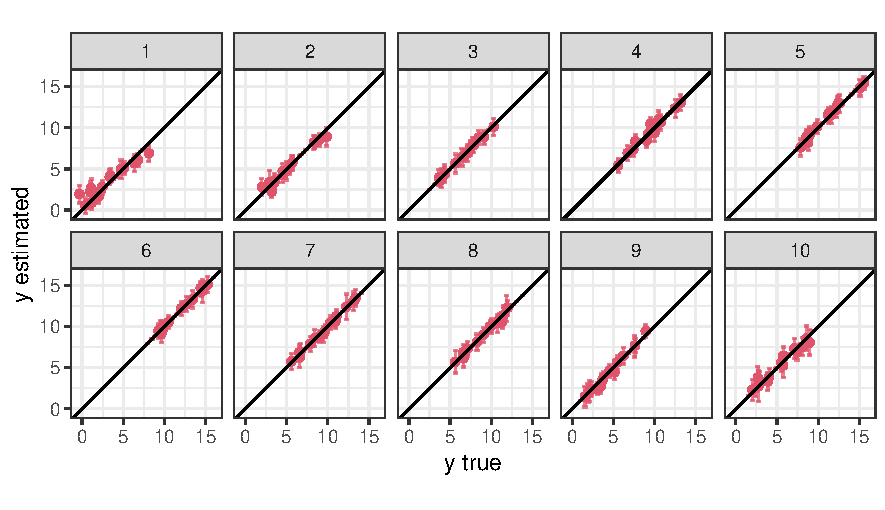
\includegraphics[width=5.0in]{./Figs/4y_true_vs_pred.pdf}
  \caption{
  Scatterplot of predicted (i.e., estimated) temperature values versus the true latent values.
The error bars represent the 95\% highest density interval, indicating the range of the most plausible true values given the predictions.
  %Predicted (i.e. estimated) temperature versus the true latent values. 
  %The error bars represent the 95\% highest density interval.
  }
  \label{figure:4y_true_vs_pred}
\end{figure}


\subsection{Predictions on a new set of prediction locations}

Environmental and ecological monitoring of stream networks often requires estimation of the response variable of interest across the whole river network.
In this section we illustrate how to use the fitted model to predict at a new set of locations using Kriging. We will produce temperature predictions at the 499 locations we generated previously using a systematic design.

\begin{example}
## Making predictions at a new set of prediction locations

## Set the seed for reproducibility
set.seed(seed)

## Extract the location IDs for prediction locations
locID_pred <- sort(unique(pred_data$locID))

## Define a new column containing the response variable used in
## fit_td, including missing values
obs_data$y_traintest <- obs_data$y

## Replace y with the original response variable, containing no
## missing values
obs_data$y <- obs_data$y_backup  

## Produce predictions: This takes approximately 8 minutes
pred <- predict(object = fit_td, ## fitted model
                path = path, #  path to .ssn object
                obs_data = obs_data, # observed data.frame
                pred_data = pred_data, # prediction data.frame
                net = 1, # network identifier (optional)
                nsamples = 100, # number of samples to use from the posterior 
                addfunccol = 'addfunccol', # variable used for spatial weights
                locID_pred = locID_pred, # location identifier for predictions
                chunk_size = 60) # split the predictions into subsets of this size

## Convert the prediction data.frame from wide to long format
ys <- reshape2::melt(pred, id.vars = c('locID0',
                                       'locID', 'date'), value.name ='y')

## Create variable representing the iteration number and set variable
## column to NULL
ys$iter <- gsub("[^0-9.-]", "", ys$variable)
ys$variable <- NULL
\end{example}

As we are using a simulated dataset, we can compare the out-of-sample predictions with the true latent values in the same way we did previously (Figure ~\ref{figure:5y_predtrue_vs_predpred}).


\begin{figure}[htbp]
  \centering
   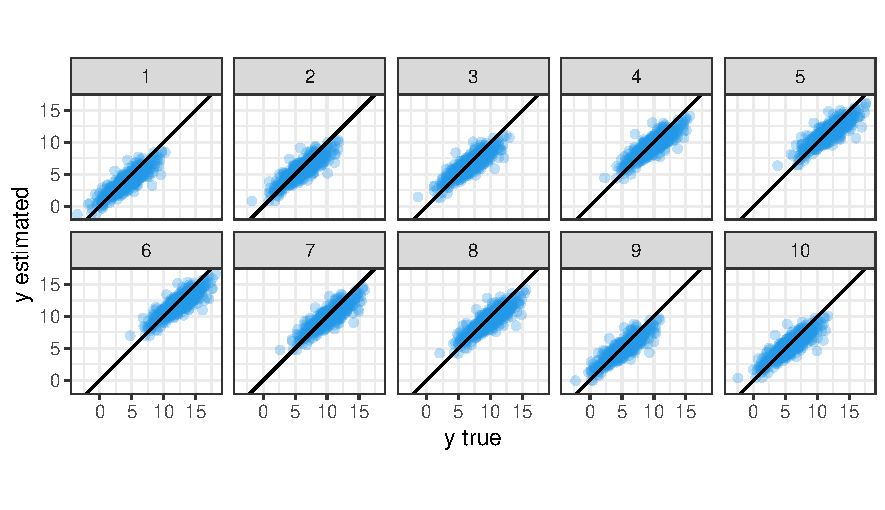
\includegraphics[width=5.0in]{./Figs/5y_predtrue_vs_predpred.pdf}
  \caption{
  Scatter plot of predicted (i.e. estimated) temperature versus the true latent values. The plot shows a strong linear relationship between the two, indicating good agreement between the true and estimated values. 
  % Predicted (i.e. estimated) temperature versus the true latent values. 
  }
  \label{figure:5y_predtrue_vs_predpred}
\end{figure}


We then visualize the posterior mean of the predictions on the full network (Figure ~\ref{figure:6network_preds}).

\begin{figure}[htbp]
  \centering
   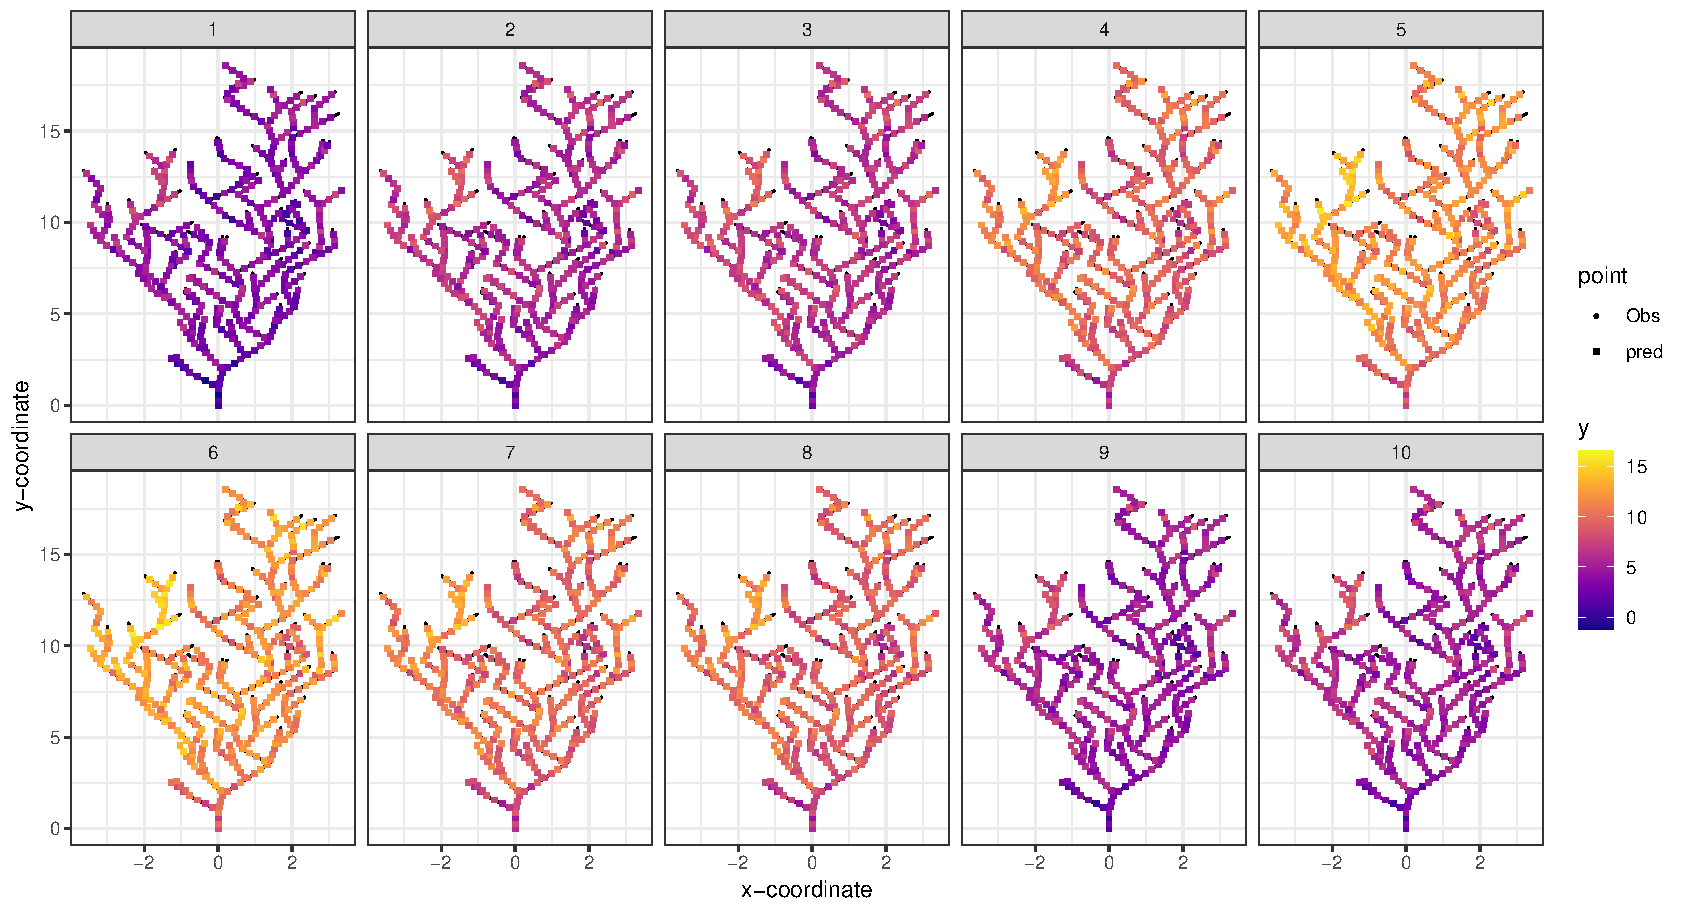
\includegraphics[width=6.0in]{./Figs/6network_preds.pdf}
  \caption{
  Evolution of observed and predicted stream temperatures over the 10 dates. The plot highlights the variability in water temperatures over time.
   %Evolution of the observed and predicted temperature over the 10 dates.
  }
  \label{figure:6network_preds}
\end{figure}



\subsection*{Exceedance probabilities throughout the network}
It is straightforward to make probabilistic statements about the predictions based on samples from the posterior predictive distribution. 
In this example, we calculate the exceedance probabilities at each prediction location based on a biological threshold of 13 \textdegree{}C. 

\begin{example}
## Computing the exceedance probabilities

## Create an exceedance indicator based on a threshold (i.e. limit)
limit <- 13
ys$exc <- ifelse(ys$y > limit , 1, 0) ## 1== TRUE, 0== FALSE

## Calculate summary statistics for the predictions, by locID and date
## and join to prediction data.frame
ys <- data.frame(ys) %>% dplyr::group_by(date, locID) %>%
  dplyr::summarise(sd = sd(y, na.rm=T), ## prediction standard deviation
                   y_pred = mean(y, na.rm=T), ## mean temperature prediction
                   prop = mean(exc, na.rm=T)) ## exceedance probability

ys <- dplyr::arrange(ys, locID)
pred_data <- pred_data %>% left_join(ys, by = c('locID', 'date'), keep = FALSE)


## Plot the exceedance probabilities for the prediction sites on 10 dates
ggplot(nets) +
  geom_path(aes(X1, X2, group = slot, size = afv_cat), lineend = 'round',
              linejoin = 'round', col = 'gray')+
  geom_point(data = dplyr::filter(pred_data) ,
             aes(x = coords.x1, y = coords.x2, col = prop), size = 1)+
  scale_size_manual(values = seq(0.2,2,length.out = 5))+
  facet_wrap(~date, nrow = 2)+
  scale_color_viridis(option = 'C')+
  scale_shape_manual(values = c(200))+
  xlab("x-coordinate") +
  ylab("y-coordinate")+
  coord_fixed()+
  theme_bw()+
  theme(axis.text=element_text(size=12),
        axis.title=element_text(size=13),
        legend.text=element_text(size=13),
        legend.title=element_text(size=13),
        strip.text.x = element_text(size = 13),
        axis.text.x = element_text(angle = 45, hjust=1),
        strip.background =element_rect(fill='white'))+
  guides(size = 'none')+
    labs(size="", colour="exceedance")
\end{example}

Figure ~\ref{figure:7network_exc_prob} shows the time series of the exceedance probabilities at prediction locations obtained from the posterior predictive distributions. Knowing when and where temperature or other water quality variables are likely  to exceed critical thresholds provides valuable information for prioritizing management and conservation activities.  


\begin{figure}[htbp]
  \centering
   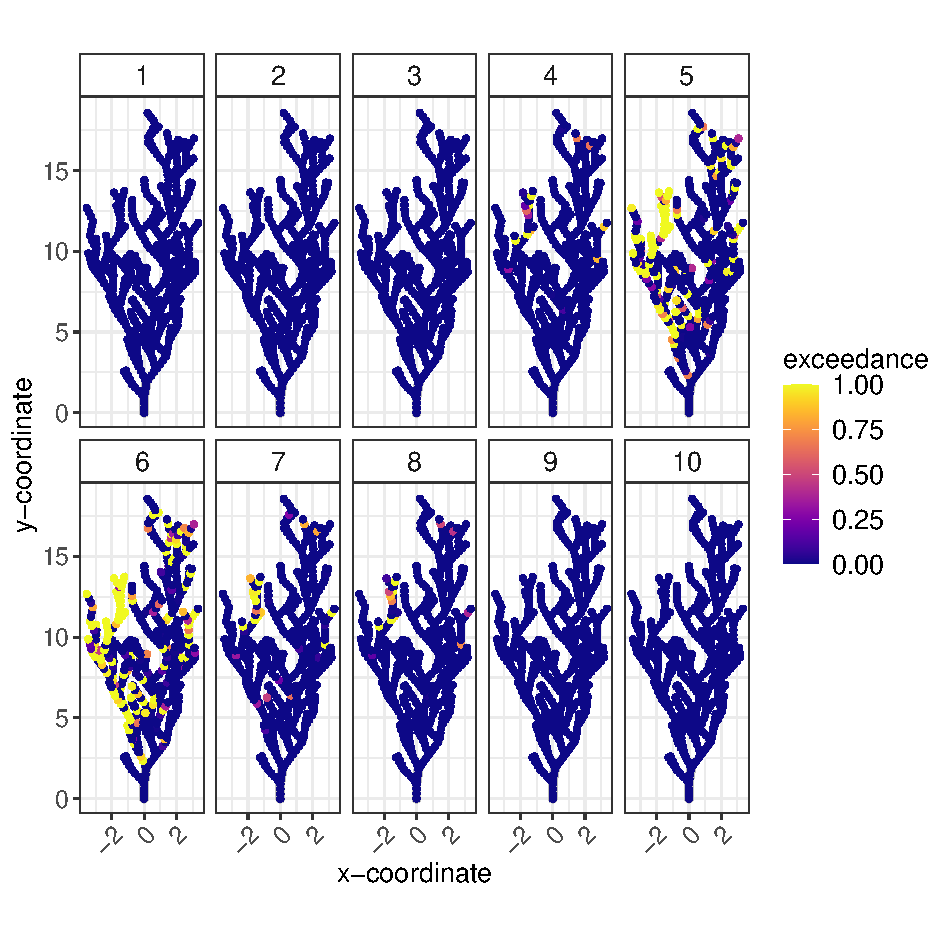
\includegraphics[width=6.0in]{./Figs/7network_exc_prob.pdf}
  \caption{
  Network exceedance probabilities across the ten dates. The yellow regions represent the areas where the probability of exceeding the limit is high.
  }
  \label{figure:7network_exc_prob}
\end{figure}


\clearpage
\section*{Other results} 
\label{sec:others}


Trace plots are often used to visually assess convergence when parameters are estimated in a Bayesian model. These can be generated easily from the \texttt{stanfit} object we saved earlier (fits) and the \texttt{traceplot} function in \CRANpkg{rstan} .

\begin{figure}[htbp]
  \centering
   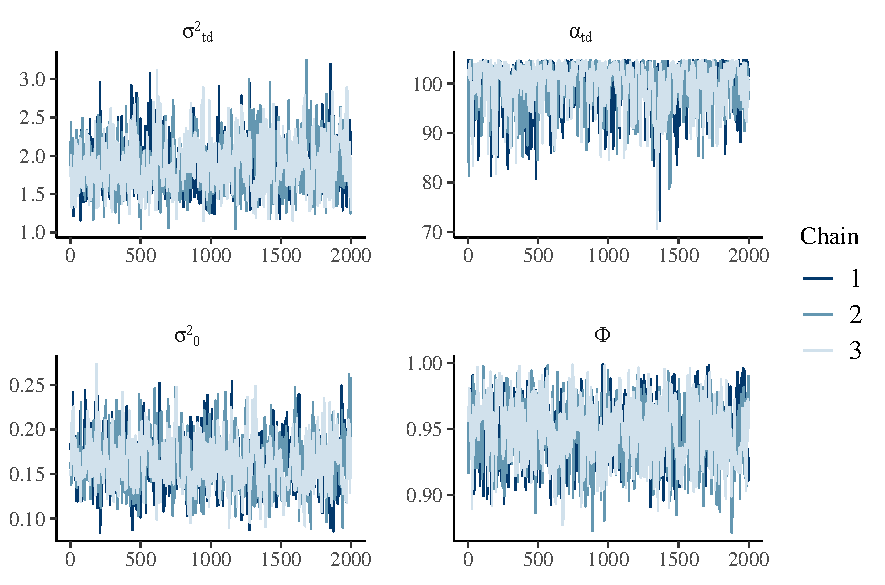
\includegraphics[width=5.0in]{./Figs/9traceplot_pars.pdf}
  \caption{Trace plots of the spatial covariance parameters including the partial sill ($\sigma^2_{TD}$), nugget effect ($\sigma^2_{0}$), range ($\alpha$), and the temporal autocorrelation parameter, $\phi$, showing good mixing of the chains. }
  \label{figure:3trace_pars}
\end{figure}



\begin{figure}[htbp]
  \centering
   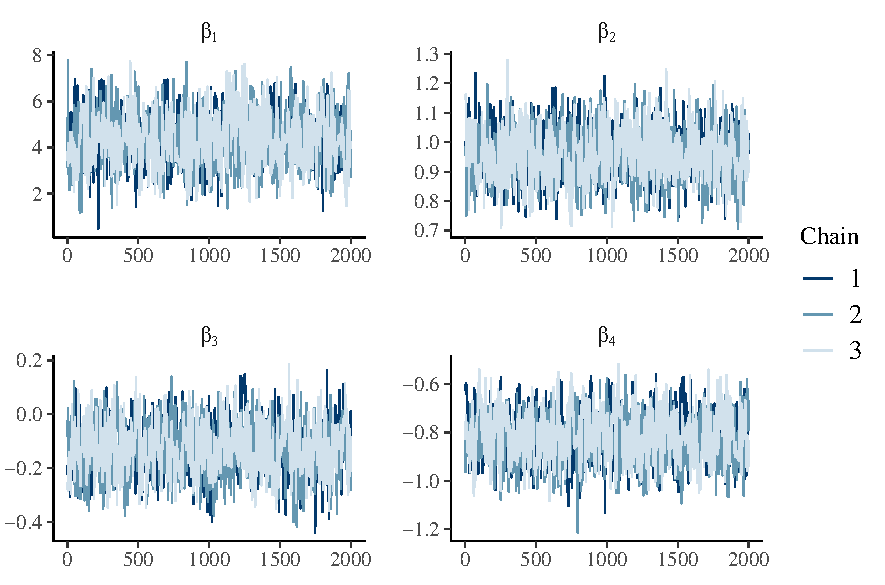
\includegraphics[width=5.0in]{./Figs/9traceplot_beta.pdf}
  \caption{Trace plots of the regression coefficients ($\beta$). }
  \label{figure:3trace_beta}
\end{figure}


\begin{figure}[htbp]
  \centering
   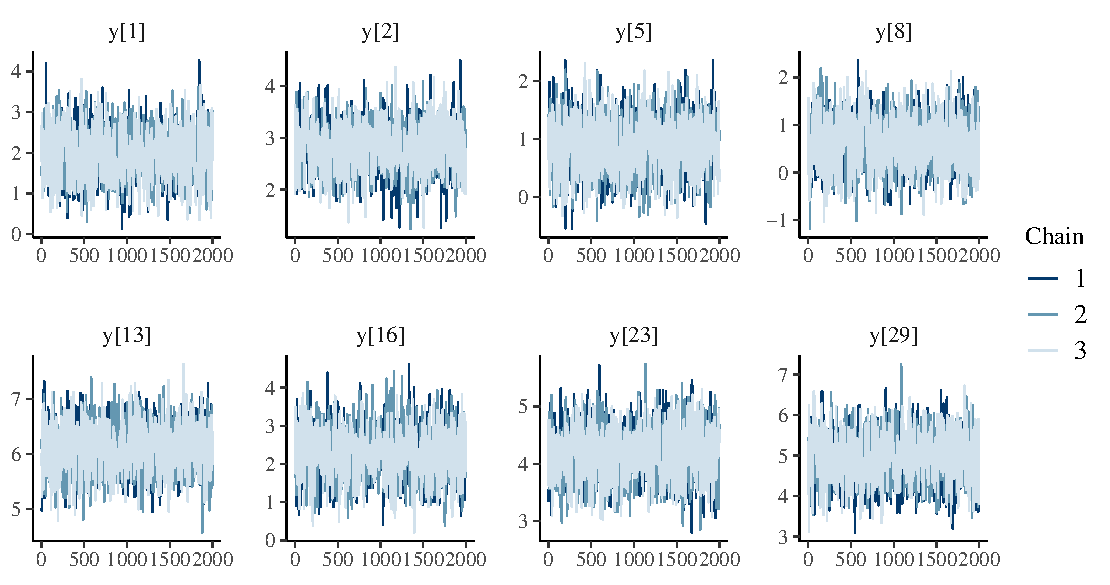
\includegraphics[width=5.0in]{./Figs/9traceplot_y.pdf}
  \caption{Trace plots of the predicted temperature ($y$) in eight prediction points. }
  \label{figure:3trace_y}
\end{figure}










\hypertarget{refs}{}

\bibliography{SSNbayes.bib}

\address{%
Edgar Santos-Fernandez\\
School of Mathematical Sciences, Queensland University of Technology\\%
Australian Research Council Centre of Excellence for Mathematical and
Statistical Frontiers (ACEMS)\\ Y Block, Floor 8, Gardens Point Campus. GPO Box 2434. Brisbane, QLD
4001.\\ Australia\\
%
%
\textit{ORCiD: \href{https://orcid.org/0000-0001-5962-5417}{0000-0001-5962-5417}}\\%
\href{mailto:santosfe@qut.edu.au}{\nolinkurl{santosfe@qut.edu.au}}%
}

\address{%
Jay M. Ver Hoef\\
Marine Mammal Laboratory, NOAA-NMFS Alaska Fisheries Science Center.\\%
Seattle, WA and Fairbanks, AK, USA\\
%
%
\textit{ORCiD: \href{https://orcid.org/0000-0003-4302-6895}{0000-0003-4302-6895}}\\%
\href{mailto:jay.verhoef@noaa.gov}{\nolinkurl{jay.verhoef@noaa.gov}}%
}

\address{%
James McGree\\
School of Mathematical Sciences, Queensland University of Technology\\%
\\
%
%
\textit{ORCiD: \href{https://orcid.org/0000-0003-2997-8929}{0000-0003-2997-8929}}\\%
\href{mailto:james.mcgree@qut.edu.au}{\nolinkurl{james.mcgree@qut.edu.au}}%
}

\address{%
Daniel J. Isaak\\
Rocky Mountain Research Station, US Forest Service\\%
\\
%
%
\textit{ORCiD: \href{https://orcid.org/0000-0002-8137-325X}{0000-0002-8137-325X}}\\%
\href{mailto:Daniel.isaak@usda.gov}{\nolinkurl{Daniel.isaak@usda.gov}}%
}

\address{%
Kerrie Mengersen\\
School of Mathematical Sciences, Queensland University of Technology\\%
Australian Research Council Centre of Excellence for Mathematical and
Statistical Frontiers (ACEMS)\\ Y Block, Floor 8, Gardens Point Campus. GPO Box 2434. Brisbane, QLD
4001.\\ Australia\\
%
%
\textit{ORCiD: \href{https://orcid.org/0000-0001-8625-9168}{0000-0001-8625-9168}}\\%
\href{mailto:k.mengersen@qut.edu.au}{\nolinkurl{k.mengersen@qut.edu.au}}%
}

\address{%
Erin E. Peterson\\
EP Consulting\\%
School of Mathematical Sciences, Queensland University of Technology\\ Australian Research Council Centre of Excellence for Mathematical and
Statistical Frontiers (ACEMS)\\ Y Block, Floor 8, Gardens Point Campus. GPO Box 2434. Brisbane, QLD
4001.\\ Australia\\
%
%
\textit{ORCiD: \href{https://orcid.org/0000-0003-2992-0372}{0000-0003-2992-0372}}\\%
\href{mailto:erin@peterson-consulting.com}{\nolinkurl{erin@peterson-consulting.com}}%
}

\end{article}


\end{document}
